% ==========================================
% Step 4/4 - Final refinement (refinement step 3)
% Output: step4-11-24-2026-tuesday-algebra_1-offset-final.tex
% Input: step3-11-24-2026-tuesday-algebra_1-offset-speech_refined.tex
% Model: gemini-4-hydrogen
% Temperature: 0.35
% TopP: 0.9
% TopK: 10
% MaxOutputTokens: 65535
% ThinkingBudget: 4096
% ThinkingLevel: HIGH
% Processed on: 2026-11-26 00:29:14
% Thought summaries: step4-11-24-2026-tuesday-algebra_1-offset-final-thoughts.md
% ------------------------------------------
% Token Usage (2 Request(s)):
%   - Total Prompt Tokens : 201'715 (gesamter Prompt, inkl. Cache)
%   - Cached Context      : 0 (aus Google Context-Cache, rabattiert)
%   - Fresh Input Tokens  : 201'715 (neu verrechneter Input)
%   - Output Tokens       : 51'048 (generiertes LaTeX, ohne Thinking)
%   - Thinking Tokens     : 21'287 (Denk-Tokens, als Output verrechnet)
% ==========================================
% ==========================================
% Step 3/4 - Speech refinement (refinement step 2)
% Output: step3-11-24-2026-tuesday-algebra_1-offset-speech_refined.tex
% Input: step2-11-24-2026-tuesday-algebra_1-offset-merged.tex
% Model: gemini-4-hydrogen
% Temperature: 0.35
% TopP: 0.9
% TopK: 10
% MaxOutputTokens: 65535
% ThinkingBudget: 4096
% ThinkingLevel: HIGH
% Processed on: 2026-11-26 00:18:55
% Thought summaries: step3-11-24-2026-tuesday-algebra_1-offset-speech_refined-thoughts.md
% Non-speech guard: all 72 segments outside speech match the input
% ------------------------------------------
% Token Usage (2 Request(s)):
%   - Total Prompt Tokens : 617'940 (gesamter Prompt, inkl. Cache)
%   - Cached Context      : 0 (aus Google Context-Cache, rabattiert)
%   - Fresh Input Tokens  : 617'940 (neu verrechneter Input)
%   - Output Tokens       : 51'185 (generiertes LaTeX, ohne Thinking)
%   - Thinking Tokens     : 34'062 (Denk-Tokens, als Output verrechnet)
% ==========================================
% ==========================================
% Step 2/4 - Merge & timestamp alignment (refinement step 1)
% Output: step2-11-24-2026-tuesday-algebra_1-offset-merged.tex
% Input: step1-11-24-2026-tuesday-algebra_1-all-offset.tex
% Model: gemini-4-hydrogen
% Temperature: 0.4
% TopP: 0.95
% TopK: 40
% MaxOutputTokens: 65535
% ThinkingBudget: 32765
% ThinkingLevel: HIGH
% Processed on: 2026-11-26 00:06:50
% Thought summaries: step2-11-24-2026-tuesday-algebra_1-offset-merged-thoughts.md
% ------------------------------------------
% Token Usage (1 Request(s)):
%   - Total Prompt Tokens : 257'155 (gesamter Prompt, inkl. Cache)
%   - Cached Context      : 0 (aus Google Context-Cache, rabattiert)
%   - Fresh Input Tokens  : 257'155 (neu verrechneter Input)
%   - Output Tokens       : 52'955 (generiertes LaTeX, ohne Thinking)
%   - Thinking Tokens     : 11'828 (Denk-Tokens, als Output verrechnet)
% ==========================================
% ==========================================
% Step 1/4 - Transcription, 4 part(s) combined
% Output: step1-11-24-2026-tuesday-algebra_1-all-offset.tex
% Source video: 11-24-2026-tuesday-algebra_1.mp4
% Model: gemini-4-hydrogen
% Temperature: 0.36
% TopP: 0.95
% TopK: 40
% MaxOutputTokens: 65535
% ThinkingBudget: 32765
% ThinkingLevel: HIGH
% Processed on: 2026-11-25 23:53:20
% ------------------------------------------
% Parts:
%   - Part 1: 11-24-2026-tuesday-algebra_1-part1.mp4 | start 00:00:00 | model gemini-4-hydrogen | processed 2026-11-25 22:35:34 | prompt 478'427 | output 15'093 | thinking 14'931 | aus Cache
%   - Part 2: 11-24-2026-tuesday-algebra_1-part2.mp4 | start 00:22:06 | model gemini-4-hydrogen | processed 2026-11-25 22:50:35 | prompt 494'180 | output 15'790 | thinking 20'432 | aus Cache
%   - Part 3: 11-24-2026-tuesday-algebra_1-part3.mp4 | start 00:44:12 | model gemini-4-hydrogen | processed 2026-11-25 23:18:26 | prompt 510'313 | output 12'383 | thinking 10'709
%   - Part 4: 11-24-2026-tuesday-algebra_1-part4.mp4 | start 01:06:18 | model gemini-4-hydrogen | processed 2026-11-25 23:53:20 | prompt 523'725 | output 16'993 | thinking 22'663
% ------------------------------------------
% Token Usage of this run (2 Request(s)):
%   - Total Prompt Tokens : 1'034'038 (gesamter Prompt, inkl. Cache)
%   - Cached Context      : 0 (aus Google Context-Cache, rabattiert)
%   - Fresh Input Tokens  : 1'034'038 (neu verrechneter Input)
%   - Output Tokens       : 29'376 (generiertes LaTeX, ohne Thinking)
%   - Thinking Tokens     : 33'372 (Denk-Tokens, als Output verrechnet)
% ==========================================

% Primary Language: English
% End of the video: 01:32:24

\lecturechapter[11]{Tuesday}{24 Nov}{24 November 2026}{Sylow's Fourth Theorem, Simple Groups, and Field Extensions}

\begin{overview}[Course Content Overview]
This lecture begins with a recap of the first three Sylow theorems and states and proves Sylow's fourth theorem, showing that the number of $p$-Sylow subgroups of a finite group is congruent to $1$ modulo $p$ via a conjugation action on the set of $p$-Sylow subgroups. It then proves that the alternating group $A_4$ of order $12$ has no subgroup of order $6$ as a counterexample to the full converse of Lagrange's theorem, introduces simple groups, proves that $A_5$ is simple while $A_4$ is not, and outlines classification hints for groups of order $p$, $p^2$, and $pq$ alongside broader directions in group theory (the classification of finite simple groups, representation theory, Klein's Erlangen program, Lie groups, and reflections on formalization and AI in mathematics). In the second half, the lecture turns to field theory and the problem of solving irreducible polynomial equations $f(\alpha) = 0$ over a field $k$, constructing the quotient field extension $K = \faktor{k[x]}{(f)}$ containing $k$ canonically and a root $\alpha = \bar{x}$ (illustrated by $\faktor{\mathbb{R}[x]}{(x^2+1)} \cong \mathbb{C}$), and proving the uniqueness theorem $K \cong k(\beta)$ for any field extension $F$ over $k$ containing a root $\beta$ of $f$.
\end{overview}

\section{Sylow's Fourth Theorem}

\subsection{Review of Sylow's Theorems and Statement of Sylow IV}

\begin{speech}[00:00:00 - 00:01:49]
Okay, so, last week was formally the end of group theory, but I wanted to say a few comments because there's some fun things to say.

So, the last topic was the Sylow theorems \inlinemetanote{writes: Sylow Theorems}. And for this, $G$ is a finite group, and we look at a prime $p^k m = n$, where this (i.e., $p^k$) is the largest prime factor (power dividing $n$) \inlinemetanote{writes \qt{$|G| = n$}, \qt{$p^k m = n$}, and \qt{$(p, m) = 1$}}.

And I remind you that the Sylow $1$ was that there exists a $p$-Sylow subgroup --- that's some subgroup inside $G$ where the size is the biggest prime (power) \inlinemetanote{writes \qt{S I:}, \qt{$\exists$ $p$-Sylow subgrp}, \qt{$P \subset G$}, and \qt{$|P| = p^k$}}.

S~II says that if $H$ has a power of $p$ and $H$ is a subgroup, then $H$ is contained in some $p$-Sylow subgroup \inlinemetanote{writes \qt{S II:}, \qt{If $|H| = p^\ell$, $H \subset G$}, and \qt{$\implies H \subset P'$ some $p$-Sylow}}.

And the third one, S~III, was that all $p$-Sylow subgroups are conjugate \inlinemetanote{writes \qt{S III:} and \qt{All $p$-Sylow subgrps $\subset G$ are conj.}}.

So, I wanted to just give you the next one, S~IV, which was what I was speaking about at the last moment of last class: this is about what is the number of $p$-Sylow subgroups of $G$ \inlinemetanote{writes \qt{S IV:} and \qt{What is number of $p$-Sylow subgrps of $G$?}}.
\end{speech}

\begin{content}[Recap of Sylow I--III and the Counting Question]
\begin{remark}[Recap: Sylow Theorems I--III]\label[remark]{rem:sylow-1-3-recap}
Let $G$ be a finite group of order $n = p^k m$, where $p$ is a prime and $(p, m) = 1$ (so $p^k$ is the highest power of $p$ dividing $n$).
\begin{itemize}
    \item \textbf{S I:} There exists a $p$-Sylow subgroup $P \subset G$ with $|P| = p^k$ (Week 10, \cref{thm:sylow-1}).
    \item \textbf{S II:} If $H \subset G$ is a subgroup with $|H| = p^\ell$, then $H \subset P'$ for some $p$-Sylow subgroup $P'$ of $G$ (\cref{thm:sylow-2}).
    \item \textbf{S III:} All $p$-Sylow subgroups of $G$ are conjugate in $G$ (\cref{thm:sylow-3}).
\end{itemize}
\end{remark}

\textbf{S IV (Question):} What is the number of $p$-Sylow subgroups of $G$? The previous lecture stated the answer (\cref{thm:sylow-4}) and left its proof as an exercise (\cref{exer:sylow-4-proof}); this lecture proves it.
\end{content}

\begin{aiNote}[Notation: \texorpdfstring{$\subset$}{subset} for Any Subgroup or Subset]
% [PERSISTENT]
As in the earlier lectures, $\subset$ is the board's sign for subsets and subgroups (Week 4, \cref{not:subset-board}).
\end{aiNote}

\begin{speech}[00:01:49 - 00:02:55]
So, we can answer this because it gives an example of a different group action we didn't have. So, we have $G$ here, we've picked our $p$, so the set of $p$-Sylow subgroups equals $V$, so this $V$ is the set of all subgroups, say $S$ in $G$, where $S$ has size $p^k$ \inlinemetanote{writes \qt{$G$}, \qt{$p$-Sylow subgrps}, \qt{$\implies V = \{$}, and \qt{$S \subset G \mid |S| = p^k \}$}}.

This is a finite set, and I want to count the number. So, this question is: what is the cardinality of this \inlinemetanote{writes: $|V| = ?$}?

And of course we're not going to get the answer to that --- it just depends on the group --- but the statement of S~IV, Sylow $4$, says that this cardinality is congruent to $1$ mod $p$ \inlinemetanote{writes and boxes: S IV: $|V| \equiv 1 \pmod p$}.

All right? And this is the last group action argument, somehow in the package, although it seems like maybe it's not exactly in the syllabus. We should put it in it.

Okay, so, we want to prove this. And the proof is an application with one new idea.
\end{speech}

\begin{content}
Let $G$ be a finite group of order $n = p^k m$ with $p$ prime and $(p, m) = 1$, and let $V$ denote the set of all $p$-Sylow subgroups of $G$:
\[
V := \left\{ S \subset G \;\big|\; |S| = p^k \right\}.
\]
We ask for the cardinality $|V|$.

\begin{highlight}{MidnightBlue}
\begin{theorem}[Sylow IV]\label[theorem]{thm:sylow-iv}
The number $|V|$ of $p$-Sylow subgroups of $G$ satisfies:
\[
|V| \equiv 1 \pmod p.
\]
\end{theorem}
\end{highlight}
\end{content}

\begin{proofWrapper}[Proof of \cref{thm:sylow-iv}]

\begin{speech}[00:02:55 - 00:04:36]
So, I want to prove this now: proof \inlinemetanote{writes: Proof:}. We start with a $p$-Sylow subgroup, with one of them \inlinemetanote{writes: Start with $P \in V$}. So, we have the subgroup $P$ inside $G$ where the order is $p^k$ \inlinemetanote{writes \qt{$P \subset G$} and \qt{$|P| = p^k$}}. Okay?

And now we're going to act on this set $V$. So, the idea in all of these Sylows is picking the right group action. Here's the idea: $G$ acts on $V$ by conjugation, meaning that if I have an element of $G$, and I have a $Q$ --- so this is an element of the group and this is a $p$-Sylow subgroup --- then I can define the action to be $g Q g^{-1}$, which is a new $p$-Sylow subgroup, or maybe new, who says \inlinemetanote{writes \qt{Idea:}, \qt{$G \curvearrowright V$ by conjug.}, \qt{$\phi(g, Q) = g Q g^{-1}$}, and \qt{$G$}, \qt{$V$}, \qt{$V$} under $g$, $Q$ and $g Q g^{-1}$, each with a small arrow pointing up}.

So, $G$ acts on the set of $p$-Sylow subgroups by conjugation. This is the crucial idea. All right?

So, do you accept this action? You have an element of $G$ and this is the set of the $p$-Sylow... and you just conjugate, you get a new $p$-Sylow subgroup. Right?

And we know various things, like Sylow $3$ (\cref{rem:sylow-1-3-recap}) says this action is transitive --- it covers all of them, I mean all $p$-Sylow subgroups are conjugate. We don't care about that now.
\end{speech}

\begin{content}[Setup and Conjugation Action on \texorpdfstring{$V$}{V}]
Start with a fixed $p$-Sylow subgroup $P \in V$, so $P \subset G$ with $|P| = p^k$.

\textbf{Idea:} The group $G$ acts on the set $V$ by conjugation ($G \curvearrowright V$):
\[
\phi \colon G \times V \to V, \qquad \phi(g, Q) = g Q g^{-1}.
\]
Indeed, since conjugation by $g \in G$ is an automorphism of $G$, $g Q g^{-1}$ is a subgroup of $G$ of the same cardinality $|g Q g^{-1}| = |Q| = p^k$, so $g Q g^{-1} \in V$.
\end{content}

\begin{speech}[00:04:36 - 00:05:24]
So, we restrict this action to this particular $p$-Sylow subgroup \inlinemetanote{writes: We restrict the action to $P \subset G$}. We get that this particular $p$-Sylow subgroup acts on the set of all $p$-Sylow subgroups by the same action, where if you take $g$ in $P$ and you take $Q$ in $V$, then this action is just the same thing, but I write it down anyway \inlinemetanote{writes \qt{$P \curvearrowright V$}, \qt{$g \in P, Q \in V$}, and \qt{$\phi(g, V) = g V g^{-1}$}, a slip for $\phi(g, Q) = g Q g^{-1}$}.

All right? So, since the whole group acts on the set, we can just look at the action of a subgroup --- in fact, this subgroup $P$, the one we chose \inlinemetanote{writes: $|P| = p^k$}.
\end{speech}

\begin{content}[Restricting the Action to \texorpdfstring{$P$}{P}]
We restrict the conjugation action of $G$ on $V$ to the chosen $p$-Sylow subgroup $P \subset G$ (with $|P| = p^k$), giving an action $P \curvearrowright V$:
\[
\phi(g, Q) = g Q g^{-1} \quad \text{for } g \in P, \; Q \in V.
\]
\end{content}

\begin{speech}[00:05:24 - 00:07:01]
Okay, so, then now we use the theorem we've used many times that when I have a group action on a set --- so this is $V$, this is the picture I drew many times last week \inlinemetanote{draws a closed curve labeled $V$, divides it by curved lines into orbits, and writes \qt{Orb decomp} below} --- it breaks it up into the orbit spaces of this group action. So, this is this orbit decomposition.

And so, we can write the equation: that's everybody in $V$ is equal to the sum of the size of the orbits \inlinemetanote{writes: $|V| =$}. And now I just skip the steps here because we did it several times, so this is the number of fixed points --- those are the orbits that are just by themselves --- then there'd be plus the size of the orbits that are not fixed points \inlinemetanote{writes: $\#$ fixed pt.}.

But those orbits that are not fixed points, their size is a power of $p$, because this thing (i.e., $P$) has order $p^k$ \inlinemetanote{points at $|P| = p^k$}. So, the orbits that are not fixed points, their sizes are powers of $p$ and not the zeroth power --- the zeroth power's been put here (i.e., in the fixed points). We did this several times.

So, the answer is that we can write this is congruent to number of fixed points mod $p$ \inlinemetanote{writes \qt{mod $p$} after it, so the line reads $|V| = \#\text{ Fixed pt} \bmod p$}. All right? I put congruent and mod $p$ twice, so maybe I just put here: it's equal to this mod $p$ (meaning congruent mod $p$). And that is the output of looking at this decomposition of $V$ in terms of orbits. The orbits have to be powers of $p$. The powers of $p$, if they're positive powers of $p$, then they're $0 \pmod p$. If they're $p^0$, they're fixed points. So, that's this equation \inlinemetanote{circles $\#$ fixed pt.}.
\end{speech}

\begin{content}[Orbit Decomposition and Fixed-Point Congruence]
\definecolor{figBlue}{HTML}{07608F} % RGB (7, 96, 143): petrol blue (MidnightBlue)
\definecolor{figGray}{HTML}{666665} % RGB (102, 102, 101): dark gray (gray!80!black)
\begin{hidden}
- Canvas: no scale, cm; oval for V centred at (0, 0) with half-axes 2.0 and 2.3, as on the board (frame 00:09:30: a closed curve labeled V, cut by curved lines into orbits, "Orb decomp" below it; no dot and no side notes on the board)
- Order: (1) fill of V (figBlue!8); (2) clipped orbit boundary curves inside V; (3) outline of V; (4) text last
- Coordinates:
  Outline: ellipse (0, 0) radii 2.0 and 2.3.
  Partition curves (drawn inside \begin{scope} \clip (0, 0) ellipse (2.0 and 2.3); ... \end{scope}):
  - (-2.1, 1.9) to (2.1, 1.9) bowing down to (0, 1.375)
  - (-2.1, 0.7) to (2.1, 0.7) bowing to (0, 0.325)
  - (-2.1, -0.4) to (2.1, -0.4) bowing to (0, -0.775)
  - (-2.1, -1.3) to (2.1, -1.3) bowing to (0, -1.6)
- Labels, inner sep=0.15cm: "V" anchor south at the top of the ellipse (0, 2.3); "orbit decomposition" anchor north at the bottom (0, -2.3)
- Collisions: none; both labels sit outside the ellipse.
\end{hidden}
\begin{center}
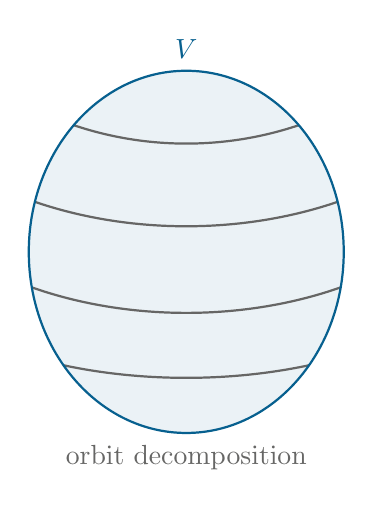
\begin{tikzpicture}
    % (1) Fill of V
    \fill[figBlue!8] (0, 0) ellipse (2.0 and 2.3);

    % (2) Orbit decomposition curves clipped to V
    \begin{scope}
        \clip (0, 0) ellipse (2.0 and 2.3);
        \draw[thick, figGray] (-2.1, 1.9) .. controls (-0.8, 1.2) and (0.8, 1.2) .. (2.1, 1.9);
        \draw[thick, figGray] (-2.1, 0.7) .. controls (-0.8, 0.2) and (0.8, 0.2) .. (2.1, 0.7);
        \draw[thick, figGray] (-2.1, -0.4) .. controls (-0.8, -0.9) and (0.8, -0.9) .. (2.1, -0.4);
        \draw[thick, figGray] (-2.1, -1.3) .. controls (-0.8, -1.7) and (0.8, -1.7) .. (2.1, -1.3);
    \end{scope}

    % (3) Outline of V
    \draw[thick, figBlue] (0, 0) ellipse (2.0 and 2.3);

    % (4) Text last
    \node[anchor=south, inner sep=0.15cm, figBlue] at (0, 2.3) {$V$};
    \node[anchor=north, inner sep=0.15cm, figGray] at (0, -2.3) {orbit decomposition};
\end{tikzpicture}
\end{center}

Decomposing $V$ into disjoint $P$-orbits yields:
\begin{equation}\label{eq:sylow4-orbit-cong}
|V| \equiv \#\text{ fixed points} \pmod p.
\end{equation}

\begin{steps}[Why Non-Fixed Orbits Vanish Modulo \texorpdfstring{$p$}{p}]
The lecture skips these steps (\qt{we did it several times}; Week 10, \cref{clm:nontrivial-orbit-size}). By the Orbit--Stabilizer Theorem (Week 9, \cref{thm:orbit-stabilizer}), the size of any $P$-orbit $\operatorname{Orb}_P(Q) = \{ g Q g^{-1} \mid g \in P \}$ divides the order of the acting group $|P| = p^k$. Thus, every orbit size is a power $p^a$ with $0 \le a \le k$:
\begin{itemize}
    \item If $a = 0$, then $|\operatorname{Orb}_P(Q)| = 1$, meaning $Q$ is a fixed point of the $P$-action.
    \item If $a \ge 1$, then $p \mid p^a = |\operatorname{Orb}_P(Q)|$, so $|\operatorname{Orb}_P(Q)| \equiv 0 \pmod p$.
\end{itemize}
Summing all orbit sizes to get $|V|$ and reducing modulo $p$ leaves only the count of fixed points in \eqref{eq:sylow4-orbit-cong}.
\end{steps}
\end{content}

\begin{hidden}
% timestamp: 00:07:01
% topic: Proof of Sylow IV: orbit decomposition of V under P-conjugation
% board_state: thm:sylow-iv, eq:sylow4-orbit-cong
% next_goal: Show that P is a fixed point and prove it is the unique fixed point in V
% open_loops: none
\end{hidden}

\begin{speech}[00:07:01 - 00:08:40]
And so, then the final claim: certainly $P$ in $V$ is a fixed point \inlinemetanote{writes: Certainly $P \in V$ is fixed pt.}.

This is now confusing, because, you know, we have this group action is $P$ cross $V$ goes to $V$, but $P$ is also a point in here (i.e., in $V$) \inlinemetanote{writes: $P \times V \to V$}. Right? Because $P$ is itself a $p$-Sylow subgroup. So, $P$ is also a point.

Here we view $P$ as a group, $V$ is the set of all $p$-Sylow subgroups, so $P$ is a point of that, and $P$ is a fixed point. You just have to look at the definitions: if I take this (i.e., $Q$) to be $P$ \inlinemetanote{points at the action formula $g Q g^{-1}$}, and I take an element in $P$, then it stays in $P$. It's kind of tautologically a fixed point.

And so, the whole proof here is we have to show that $P$ in $V$ is the unique fixed point \inlinemetanote{writes: Show that $P \in V$ is Unique fixed pt.}. So, it's kind of a nice argument also.

This proof is going to show that actually the number of fixed points \inlinemetanote{draws an arrow from the circled \qt{\# Fixed pt} to a \qt{$1$}}, this is actually just $1$. And so, you get the number of $p$-Sylow subgroups is $1 \pmod p$.

Right? So, the crucial thing here is to show that this action on the set of $p$-Sylow subgroups by one $p$-Sylow subgroup has a unique fixed point, and that unique fixed point is that $p$-Sylow subgroup. That's what you have to show. And that also has a clever argument, which I give.
\end{speech}

\begin{content}[Goal: Uniqueness of the Fixed Point]
Certainly $P \in V$ is a fixed point of the action $P \times V \to V$ (note the dual role of $P$, both as the acting group and as an element of $V$): for every $g \in P$, since $P$ is a subgroup, we have $g P g^{-1} = P$.

It therefore suffices to show that $P \in V$ is the \emph{unique} fixed point of $P \curvearrowright V$; this will give $\#\text{ fixed points} = 1$, and \eqref{eq:sylow4-orbit-cong} will immediately yield $|V| \equiv 1 \pmod p$.
\end{content}

\begin{speech}[00:09:00 - 00:09:49]
That's nice because we didn't really use the conjugation action so much last week. We used very much the translation action, the left action of $G$ on itself, but this part of the argument uses the conjugation action.

Which, as I said, if you have a group, you have two actions that are given immediately, which is the conjugation action and the left action. And in this Sylow theory, both play a role. \inlinemetanote{erases the lower board}
\end{speech}

\begin{speech}[00:09:49 - 00:10:21]
Okay, so, that's the last thing we have to prove, that it's a unique fixed point.

Here is: suppose $Q$ in $V$ is a fixed point for this $P$-action on $V$ \inlinemetanote{writes: Suppose $Q \in V$ is a fixed pt. for $P \curvearrowright V$}. Right? So, of course, we must prove actually this $p$-Sylow subgroup is equal to $P$ \inlinemetanote{writes and boxes: We must prove $Q = P$}. That's the goal.
\end{speech}

\begin{content}[Uniqueness Setup]
Suppose $Q \in V$ is a fixed point for the action $P \curvearrowright V$. We must prove that $Q = P$.
\end{content}

\begin{speech}[00:10:21 - 00:11:22]
And the clever construction is: so we look at $Q$, this is our $p$-Sylow subgroup \inlinemetanote{writes: $Q \subset G$}. The clever idea here is let $N$ inside $G$ be --- this is the new definition --- the normalizer of $Q$ \inlinemetanote{writes: $N \subset G$ be the normalizer of $Q$}.

So, I have to define this. This is the definition: $N$ is equal to the set of elements $x$ in $G$ such that $x Q x^{-1}$ is equal to $Q$ \inlinemetanote{writes: $N \stackrel{\text{def}}{=} \{ x \in G \mid x Q x^{-1} = Q \}$}. All right? That's the definition of the normalizer of this set.

Sometimes this is written as $N(Q)$, or sometimes it's written as $\operatorname{Norm}(Q)$ \inlinemetanote{writes: $N(Q)$, $\operatorname{Norm}(Q)$}. The word \qt{norm} --- anything with norm is like the most overused word in mathematics --- everything's called normalizer. Anyway, this is the normalizer. That's the definition.
\end{speech}

\begin{content}[The Normalizer of \texorpdfstring{$Q$}{Q}]
\begin{definition}[Normalizer of \texorpdfstring{$Q$}{Q}]\label[definition]{def:normalizer}
Let $Q \subset G$. The \newterm{normalizer} of $Q$ in $G$, denoted $N$ (also written $N(Q)$ or $\operatorname{Norm}(Q)$), is defined as:
\[
N \stackrel{\text{def}}{=} \left\{ x \in G \;\big|\; x Q x^{-1} = Q \right\}.
\]
\end{definition}
\end{content}

\begin{speech}[00:11:22 - 00:12:10]
All right? And a little lemma, which I leave for you --- and it's hardly going to be a surprise --- is: $N$ inside $G$... \inlinemetanote{writes: Lemma: $N \subset G$ is a} what am I going to write here? \inlinemetanote{inaudible response from a student} Yeah. Is a subgroup, yeah \inlinemetanote{writes: subgroup}. Why? Because if $x$ is the identity, it's in here, and this equation is okay with composition and inverse, so...

So, that's a little lemma for you to check, it's a subgroup. What do we have here?

And the next lemma is that $Q$ is in $N$ \inlinemetanote{writes: Lemma: $Q \subset N$}. Well, that's just by definition, because $Q$ is a subgroup, so this stuff stays inside $Q$.

So, we always have $Q$ inside $N$ inside $G$ \inlinemetanote{writes: $Q \subset N \subset G$}.
\end{speech}

\begin{content}[Properties of the Normalizer]
\begin{lemma}\label[lemma]{lem:normalizer-subgroup}
$N \subset G$ is a subgroup.
\end{lemma}
\begin{proof}[Proof Sketch]
The identity $e \in G$ satisfies $e Q e^{-1} = Q$, so $e \in N$. If $x, y \in N$, then $(xy) Q (xy)^{-1} = x (y Q y^{-1}) x^{-1} = x Q x^{-1} = Q$ (closure), and $x^{-1} Q x = x^{-1} (x Q x^{-1}) x = Q$ (inverses). Thus, $N \subset G$ is a subgroup.
\end{proof}

\begin{lemma}\label[lemma]{lem:q-in-normalizer}
$Q \subset N$, and hence we have the chain of subgroups $Q \subset N \subset G$.
\end{lemma}
\begin{proof}
Since $Q$ is a subgroup of $G$, for every $x \in Q$ we have $x Q x^{-1} = Q$, which means $x \in N$.
\end{proof}
\end{content}

\begin{speech}[00:12:10 - 00:13:08]
But now, remember: this (i.e., $G$) has order $p^k m$, where $m$ is relatively prime to $p$, and this (i.e., $Q$) has order $p^k$, because it's a $p$-Sylow subgroup, right \inlinemetanote{writes \qt{$p^k m$} under $G$ and \qt{$p^k$} under $Q$}?

That means all of the powers of $p$ are already here (i.e., in $Q$). The order of $N$ divides the order of $G$. That's a fact --- I mean, we proved that, it's Lagrange. So, then there can't be any more powers of $p$ in $N$ than in $G$, because order of $N$...

So, the conclusion of this is that $Q$ is also a $p$-Sylow subgroup of $N$ \inlinemetanote{writes: $Q$ is also a $p$-Syl. of $N$}. $N$ is a group in its own right, and it has its own $p$-Sylow subgroups, and $Q$ has to be one, because it's a subgroup of $N$ of the highest power of $p$. Do you agree with this?
\end{speech}

\begin{content}[\texorpdfstring{$Q$}{Q} as a \texorpdfstring{$p$}{p}-Sylow Subgroup of \texorpdfstring{$N$}{N}]
In the chain $Q \subset N \subset G$, we know $|Q| = p^k$ and $|G| = p^k m$ with $(p, m) = 1$. By Lagrange's Theorem (Week 7, \cref{thm:lagrange}), $|Q|$ divides $|N|$ and $|N|$ divides $|G| = p^k m$. Consequently, $p^k$ is also the highest power of $p$ dividing $|N|$, which means $Q$ is a $p$-Sylow subgroup of $N$.
\end{content}

\begin{hidden}
% timestamp: 00:13:08
% topic: Proof of Sylow IV: Q and P inside the normalizer N of Q
% board_state: def:normalizer, lem:normalizer-subgroup, lem:q-in-normalizer
% next_goal: Show P is also a p-Sylow subgroup of N and apply Sylow III in N to conclude P = Q
% open_loops: none
\end{hidden}

\begin{speech}[00:13:08 - 00:13:50]
Since $Q$ is a fixed point, this implies that $P$ is also a $p$-Sylow subgroup of $N$ \inlinemetanote{writes \qt{Since $Q$ is $P \curvearrowright V$ fixed pt $\implies$} and \qt{$P$ is also $p$-Syl. of $N$}}.

Since it's a fixed point, any element of $P$ satisfies this equation (i.e., $x Q x^{-1} = Q$). So, all of $P$ is inside here (i.e., $N$). We have this picture: we have $N$ inside $G$, and both $Q$ and $P$ are inside $N$, and they're both $p$-Sylow subgroups of $N$ \inlinemetanote{writes: $Q, P \subset N \subset G$}. Okay? This argument's about to end, and it'll end in a surprising way.
\end{speech}

\begin{content}[\texorpdfstring{$P$}{P} as a \texorpdfstring{$p$}{p}-Sylow Subgroup of \texorpdfstring{$N$}{N}]
Since $Q$ is a fixed point under $P$-conjugation, every $x \in P$ satisfies $x Q x^{-1} = Q$, which by \cref{def:normalizer} means $P \subset N$. Since $|P| = p^k$, $P$ is also a $p$-Sylow subgroup of $N$. Thus, both $P$ and $Q$ are $p$-Sylow subgroups of $N$ ($Q, P \subset N \subset G$).
\end{content}

\begin{speech}[00:13:50 - 00:14:47]
So, now we apply Sylow $3$ to $N$ \inlinemetanote{writes: Apply S III to $N$}. What does Sylow $3$ say to $N$? It says that all $p$-Sylow subgroups of $N$ are conjugate. So, that means these two groups have to be conjugate inside $N$.

That means $P$ and $Q$ are conjugate in $N$ \inlinemetanote{writes: $\implies$ $P, Q$ are conj. in $N$}.

So, that's a remarkable statement, but what is $N$? $N$ is the set of people (elements) that leave $Q$ invariant. So, if $P$ and $Q$ are conjugate inside $N$, $P$ must equal $Q$ \inlinemetanote{writes: $\implies P = Q$}.

That's a beautiful argument also at the end. Because that's exactly what $N$ is: $N$ is the ones where the conjugation is just itself. So, you couldn't get anything more. So, that's Sylow $4$.
\end{speech}

\begin{content}[Conclusion: \texorpdfstring{$P = Q$}{P = Q}]
Applying Sylow III (\cref{thm:sylow-3}) to the group $N$, all $p$-Sylow subgroups of $N$ are conjugate in $N$. Therefore, $P$ and $Q$ are conjugate in $N$: there exists $x \in N$ such that
\[
P = x Q x^{-1}.
\]
However, by the definition of the normalizer $N$ (\cref{def:normalizer}), every $x \in N$ satisfies $x Q x^{-1} = Q$. It follows immediately that $P = Q$.

Hence, $P \in V$ is the unique fixed point of the $P$-action on $V$, so $|V| \equiv 1 \pmod p$, completing the proof of \cref{thm:sylow-iv}.

\begin{steps}[Summary of the Uniqueness Argument]
To prove any fixed point $Q$ of $P \curvearrowright V$ equals $P$, the argument embeds both $P$ and $Q$ into the normalizer $N = N(Q)$. Both have order $p^k$ and are therefore $p$-Sylow subgroups of $N$. By Sylow III applied to $N$, they must be conjugate by some element of $N$ --- yet every element of $N$ fixes $Q$ under conjugation, forcing $P = Q$.
\end{steps}
\end{content}

\end{proofWrapper}

\begin{speech}[00:14:47 - 00:15:33]
And I wanted to say a couple more things about groups \inlinemetanote{raises the lower chalkboard and erases the bottom board}.

But this is a fun argument. It has some new ideas in it. So, now you know Sylow $1, 2, 3$, and $4$. As far as I could tell, only Sylow $1, 2$, and $3$ are on the syllabus, so $4$ is extra for you. Right.

So, I said some things quickly last week, and I wanted to be a little more explicit about them, because they also have ideas about how to think about groups.
\end{speech}

\section{Counterexample to the Full Converse of Lagrange's Theorem: \texorpdfstring{$A_4$}{A4}}

\begin{speech}[00:15:33 - 00:16:55]
So, I said that the Sylow theory was a partial converse to Lagrange. This Lagrange's theorem says if you have a subgroup, it has to divide the order of the group. Sylow says that for certain divisors, there exist subgroups.

So, what's an example of a group that has a divisor of its order that's not represented by a subgroup \inlinemetanote{writes \qt{What is example of group} and stops}? What is an example of a group, and the example I gave is $A_4$, this is order $12$.

Maybe I should reform this, just give you the example. It's logically easier. Consider $A_4$, and that has order $12$, and the claim is that $A_4$ does not have a subgroup of order $6$ \inlinemetanote{erases \qt{What is example of group} and writes \qt{Consider $|A_4| = 12$} and \qt{Claim is that $A_4$ does not have a subgroup of order $6$.}}.

Okay? So, this says that the full converse to Lagrange is impossible. The full converse to Lagrange would say that any time I have a finite group and I take a divisor, there exists a subgroup --- that would be the full converse --- and this example shows that is impossible.
\end{speech}

\begin{content}
\recap{The previous lecture left this as an exercise (Week 10, \cref{exer:a4-no-order-6}).}

While Sylow's theorems provide a partial converse to Lagrange's theorem (Week 10, \cref{rem:partial-converse-lagrange}), the full converse is false.

\begin{proposition}[No Subgroup of Order \texorpdfstring{$6$}{6} in \texorpdfstring{$A_4$}{A4}]\label[proposition]{prop:a4-no-order-6}
Consider the alternating group $A_4$, which has order $|A_4| = 12$. Then $A_4$ does not have a subgroup of order $6$.
\end{proposition}
\end{content}

\begin{proofWrapper}[Proof of \cref{prop:a4-no-order-6}]

\begin{speech}[00:16:55 - 00:18:17]
All right, and I said that you could check this by brute force, and that was kind of a joke. You can't really check it... well, you know. There's a very simple way to think about this, this particular example. And this is kind of the hallmark of group theory: there's always these different kinds of arguments for everything. It's an interesting subject.

So, suppose $H$ inside $A_4$ has order $6$ \inlinemetanote{writes: Suppose $H \subset A_4$ has $|H| = 6$}.

All right, so, I want to rule this out, so I'm going to suppose this exists and later, you know, find some contradiction. The first thing is that then $H$ inside $A_4$ would have to be normal \inlinemetanote{writes: Then $H \subset A_4$ would have to be normal}.

And why is that? Because it was a comment I made in an earlier lecture that any time I have a finite subgroup --- sorry, a finite group and a subgroup of half the order, it has to be normal. This was a comment I made in lecture, and so that's a fact.

It's easy to prove, and you should think about it if you did not understand the comment when I made it. Has to be normal. That helps a lot, because we're trying to show it doesn't exist, so we want to pile up all properties, more and more properties on it until we can rule it out.
\end{speech}

\begin{content}[Normality of an Index-\texorpdfstring{$2$}{2} Subgroup]
Suppose for contradiction that there exists a subgroup $H \subset A_4$ with $|H| = 6$.

Since $|H| = 6 = \frac{1}{2}|A_4|$ (so $H$ has index $2$ in $A_4$), $H$ would have to be a normal subgroup of $A_4$, by the comment from an earlier lecture (Week 9, \cref{prop:index-2-normal}).
\end{content}

\begin{speech}[00:18:17 - 00:18:45]
So, if it's normal, then the next observation is that $H$ must then be a union of conjugacy classes of $A_4$ \inlinemetanote{writes: $H$ must then be a union of Conj. classes of $A_4$}.

Because a normal subgroup --- if you have an element of a normal subgroup, then all the conjugacy class has to fit in it, because remember, normality means it's invariant under conjugation.
\end{speech}

\begin{content}[Union of Conjugacy Classes]
Because $H$ is normal in $A_4$, it is invariant under conjugation ($g H g^{-1} = H$ for all $g \in A_4$; Week 8, \cref{rem:normal-conjugate-closed}). Therefore, whenever an element lies in $H$, its entire conjugacy class in $A_4$ must lie in $H$. Consequently, $H$ must be a union of conjugacy classes of $A_4$.
\end{content}

\begin{hidden}
% timestamp: 00:18:45
% topic: Proof that A_4 has no subgroup of order 6 via conjugacy classes
% board_state: prop:a4-no-order-6
% next_goal: List conjugacy class sizes of A_4 and check that no union containing (1) has size 6
% open_loops: none
\end{hidden}

\begin{speech}[00:18:45 - 00:20:42]
So, we have to think about $A_4$: what are the conjugacy classes \inlinemetanote{writes: $A_4$}? Well, of course, there's the neutral element, and that has conjugacy class of size $1$ \inlinemetanote{writes $(e)$ with a downward arrow and \qt{$1$}}.

Then there's elements that look like this and their conjugates \inlinemetanote{writes $(12)(34)$ with a downward arrow}. How many of these are there? So, how many elements in $A_4$ are conjugate to this, you have to think about all the ways... Yeah? \inlinemetanote{inaudible response from a student} Three, because you can write this in three ways. You can check that yourself: three \inlinemetanote{writes: $3$}.

Then, an interesting question is that then there's the conjugacy class of $3$-cycles --- that's also even, these are even \inlinemetanote{writes $(123)$ with a downward arrow}. This is a harder question, I'll tell you the answer: there's actually $8$ of these. So, there's $8$ elements like this, because there's $4$ choose $3$, which is $4$, and then there's two ways to put a $3$-cycle, so there's $8$ of them. And they're all conjugate in $S_4$, but $S_4$ is not $A_4$. It's harder to be conjugate in $A_4$ because you have fewer elements to conjugate with. And it turns out that this breaks up into two conjugacy classes of $4$ and $4$ \inlinemetanote{draws two arrows down from $(123)$ and writes \qt{$4$} under each}. And this better add up to $12$, which it does.

So, these are the sizes of the conjugacy classes in $A_4$. One thing you have to check is that for here, there's $8$ cycles that look like this, but they break up into two conjugacy classes, and you have to check that one way or the other.

So, this is the way the conjugacy classes break, and you see that you cannot take any sum of these numbers and get $6$, you can't do it. So, no combination has $6$ elements \inlinemetanote{writes: No comb. has $6$ elements.}.

Running the logic: if there were a subgroup of order $6$, it would have to be normal. If it's normal, it would have to be a union of conjugacy classes, and so it would have to be that in this set I could pick some subsets that add up to $6$, and it's not possible. You can just check. You can try.
\end{speech}

\begin{content}[Conjugacy Class Sizes of \texorpdfstring{$A_4$}{A4}]
The conjugacy classes of $A_4$ have the following sizes (as on the board):
\begin{center}
\begin{tabular}{c c c c}
\toprule
$(e)$ & $(12)(34)$ & \multicolumn{2}{c}{$(123)$} \\
$\downarrow$ & $\downarrow$ & $\swarrow$ & $\searrow$ \\
$1$ & $3$ & $4$ & $4$ \\
\bottomrule
\end{tabular}
\end{center}
The eight $3$-cycles are all conjugate in $S_4$, but in $A_4$ there are fewer elements available to conjugate by, and they split into two conjugacy classes of size $4$ each (left to the students to check).

No combination of these conjugacy class sizes sums to $6$:
\[
1 + 3 = 4, \quad 1 + 4 = 5, \quad 1 + 3 + 4 = 8, \quad 1 + 4 + 4 = 9, \quad 1 + 3 + 4 + 4 = 12
\]
(and $H$ must contain the identity $(e)$ of class size $1$; even without that, $\{3, 4, 4\}$ cannot sum to $6$). This contradiction shows that $A_4$ has no subgroup of order $6$.

\begin{steps}[Why the \texorpdfstring{$3$}{3}-Cycles Split in \texorpdfstring{$A_4$}{A4}]
Going beyond the lecture: the elements of $S_4$ that commute with $(123)$ form the subgroup $\langle (123) \rangle$ of order $3$, which lies in $A_4$. By the Orbit--Stabilizer Theorem for the conjugation action of $A_4$ on itself (Week 9, \cref{thm:orbit-stabilizer}), the conjugacy class of $(123)$ in $A_4$ has $12 / 3 = 4$ elements, namely $(123)$, $(134)$, $(142)$, $(243)$, and the same count holds for every $3$-cycle. So the eight $3$-cycles form two classes of four. The other class contains $(132)$: the elements of $S_4$ that conjugate $(123)$ into $(132)$ form the coset $(23)\langle (123) \rangle$, and all of them are odd permutations.
\end{steps}
\end{content}

\end{proofWrapper}

\begin{speech}[00:20:42 - 00:21:38]
So, that's the non-brute-force way. And if you understand this argument, you can prove something else, which is kind of crucial for Algebra $2$, which I mention here \inlinemetanote{raises the $A_4$ board and erases the lower board}.
\end{speech}

\section{Simple Groups and the Simplicity of \texorpdfstring{$A_5$}{A5}}

\begin{speech}[00:21:38 - 00:22:28]
So, here we were lucky because we were searching for any subgroup, it just happened that a subgroup of order $6$ had to be normal, so we could use properties of normal subgroups, which is easier to handle.

So, the natural generalization of this argument --- let's do it for $A_5$. It's a definition: $G$ is a simple --- it's a definition of this term, \newterm{simple} --- finite group, well let's just say doesn't have to be finite, simple group, and this is the definition: $G$ has no non-trivial normal subgroups \inlinemetanote{writes \qt{Def.}, \qt{$G$ is a simple} (underlined), \qt{finite}, then erases \qt{finite} and writes \qt{group}, a vertical double arrow marked \qt{def}, and \qt{$G$ has no nontrivial Normal Subgroups.}}.

Because always the neutral element and all of $G$, they're always normal subgroups, so if it's simple, it has no non-trivial normal subgroups. All right?
\end{speech}

\begin{content}
\begin{definition}[Simple Group]\label[definition]{def:simple-group}
A group $G$ is a \newterm{simple group} $\stackrel{\text{def}}{\iff}$ $G$ has no non-trivial normal subgroups (i.e., its only normal subgroups are $\{e\}$ and $G$).
\end{definition}
\end{content}

\begin{speech}[00:22:28 - 00:22:42]
And the proposition that is very useful in Algebra $2$ is that the group we've seen, $A_5$, is simple \inlinemetanote{writes \qt{Prop.} and \qt{$A_5$ is simple.}}.
\end{speech}

\begin{content}
\begin{proposition}[\texorpdfstring{$A_5$}{A5} is Simple]\label[proposition]{prop:a5-simple}
The alternating group $A_5$ is simple.
\end{proposition}
\end{content}

\begin{proofWrapper}[Proof of \cref{prop:a5-simple}]

\begin{speech}[00:22:42 - 00:24:15]
So, I want to prove this now: proof \inlinemetanote{writes: Proof.}. This group $A_5$, we discussed it, it's a group of order $60$, and the claim is it has no non-trivial normal subgroups \inlinemetanote{writes: $|A_5| = 60$.}. Not that it doesn't have subgroups: it has subgroups, but none of them are normal.

So, how could we prove this? Well, there's a strategy there: if $H$ in $A_5$ were a normal subgroup, $H$ would have to be a union of conjugacy classes of $A_5$, just like we had here (i.e., for $A_4$) \inlinemetanote{writes \qt{If $H \subset A_5$ were normal subgroup,} and \qt{$H$ would have to be a union of conj. classes of $A_5$}}.

So, now we need to figure out... There's two things $H$ would have to be: it'd have to be a union of conjugacy classes, and of course its order would have to divide $60$, because if it's a subgroup it has to have order dividing $60$. So, we just have to see whether we can find some conjugacy classes that their union is a size that divides $60$. All right?

Now you have to find the conjugacy classes in $A_5$ \inlinemetanote{writes: Find conj. classes of $A_5$}. We did this in $A_4$, but you can do it on your own time. There's different ways to do it, but it requires playing. It's not like a pure thought discussion at this point: you have to find them.
\end{speech}

\begin{content}[Conjugacy Class Strategy for \texorpdfstring{$A_5$}{A5}]
We have $|A_5| = \frac{5!}{2} = 60$. If $H \subset A_5$ were a normal subgroup, then:
\begin{enumerate}[label=\textbf{(\arabic*)}]
    \item $H$ would have to be a union of conjugacy classes of $A_5$ (since normal subgroups are closed under conjugation), and
    \item $|H|$ would have to divide $|A_5| = 60$ (by Lagrange's Theorem).
\end{enumerate}
Thus, to check whether a proper non-trivial normal subgroup $H$ can exist, we determine the sizes of the conjugacy classes of $A_5$.
\end{content}

\begin{speech}[00:24:15 - 00:25:12]
And the way to do this is that, to first order, you should think about them: they're probably very close to the conjugacy classes of $S_5$, which have to do with partitions. So, you take those and then you see the conjugation in $A_5$ is slightly weaker, because you can only conjugate by even things. So, you have to see what happens.

And I'll just tell you what the answers are here, if I can remember: $1$... the conjugacy classes are of this order, and the last one splits, so it should be like that \inlinemetanote{writes \qt{$1,$}, \qt{$15, 20,$}, and \qt{$12, 12$}}. So, hopefully this adds up to $60$, which it does.

So, that's the order of the conjugacy classes. This is for you to check \inlinemetanote{draws arrow from $1, 15, 20, 12, 12$ and writes: for you to check}. And this is a finite check, and it's not a very hard one, but just like we did for $A_3$ (slip for $A_4$), you have to do a little bit of work and playing with the group. There's no way around that. Because after all, this is a property of this group. You have to use something about this group.
\end{speech}

\begin{content}[Conjugacy Class Sizes of \texorpdfstring{$A_5$}{A5}]
The sizes of the conjugacy classes of $A_5$ are:
\[
1, \quad 15, \quad 20, \quad 12, \quad 12
\]
(which sum to $1 + 15 + 20 + 12 + 12 = 60 = |A_5|$, left as an exercise to verify).

\begin{steps}[Origin of the Class Sizes from \texorpdfstring{$S_5$}{S5}]
Going beyond the lecture: the even permutations in $S_5$ have cycle types $(1)$, $(12)(34)$, $(123)$, and $(12345)$, of sizes $1$, $15$, $20$, and $24$ respectively. The $15$ double transpositions and $20$ $3$-cycles remain single conjugacy classes in $A_5$, whereas the $24$ $5$-cycles split into two $A_5$-conjugacy classes of size $12$ each.
\end{steps}
\end{content}

\begin{hidden}
% timestamp: 00:25:12
% topic: Proof that A_5 is simple using conjugacy class sizes
% board_state: def:simple-group, prop:a5-simple
% next_goal: Conclude that no proper divisor of 60 can be formed from the class sizes including 1
% open_loops: none
\end{hidden}

\begin{speech}[00:25:12 - 00:25:52]
All right, so, then the claim is that we have to now take some summands of these numbers and get something that divides $60$, right? So, you could say, \qt{Ah, I could just take this one \inlinemetanote{points at $15$ or $12$}.}

But the point is it has to be a summand which includes the neutral element, because the subgroup has to have the neutral element. So, it has to have this $1$ in it \inlinemetanote{marks $1$}, and you have to take this $1$ and take some of these \inlinemetanote{gestures over $15, 20, 12, 12$} and get some number that divides $60$.

And you can't do it, actually. So, this $H$ doesn't exist \inlinemetanote{writes: $H$ doesn't exist!}.
\end{speech}

\begin{content}[Non-Existence of Non-Trivial Normal Subgroups]
Any subgroup $H \subset A_5$ must contain the neutral element $e$, whose conjugacy class has size $1$. Thus, $|H|$ must be a sum of a subset of $\{1, 15, 20, 12, 12\}$ containing $1$, and must also divide $60$.

No such proper non-trivial sum divides $60$, so a proper non-trivial normal subgroup $H$ does not exist.

\begin{steps}[Checking the Proper Sums]
Going beyond the lecture: the possible sums of subsets of $\{1, 15, 20, 12, 12\}$ that include $1$ and at least one other class size are:
\begin{align*}
1 + 12 &= 13, & 1 + 15 &= 16, & 1 + 20 &= 21, \\
1 + 12 + 12 &= 25, & 1 + 12 + 15 &= 28, & 1 + 12 + 20 &= 33, \\
1 + 15 + 20 &= 36, & 1 + 12 + 12 + 15 &= 40, & 1 + 12 + 12 + 20 &= 45, \\
1 + 12 + 15 + 20 &= 48.
\end{align*}
None of these numbers divides $60$. Hence, the only possibilities for $|H|$ are $1$ and $60$, proving that $A_5$ is simple.
\end{steps}
\end{content}

\end{proofWrapper}

\begin{speech}[00:25:52 - 00:26:34]
You could say, \qt{Well, what about here \inlinemetanote{points up to the $A_4$ table on the upper board}?} Were there any normal... I didn't say that there were no normal subgroups here (i.e., in $A_4$). And again, you'd have to find some combination of $1, 3, 4$, and $4$ that contains the $1$, because it has to have the neutral element, and divides $12$. So, can you do that? And the answer is yes, you can take the $1 + 3$.

So, that says it's possible: a candidate for a normal subgroup of $A_4$ would be the neutral element and all these products of two cycles, and that is true --- it is a subgroup, and it's a normal subgroup. So, $A_4$ is not simple.

But $A_5$ you can't do it. Okay, so, that was a second thing. In Galois theory this is an important point.
\end{speech}

\begin{content}
\begin{remark}[Non-Simplicity of \texorpdfstring{$A_4$}{A4}]\label[remark]{rem:a4-not-simple}
Unlike $A_5$, the group $A_4$ of order $12$ (with conjugacy class sizes $1, 3, 4, 4$) does admit a proper non-trivial sum containing $1$ that divides $12$, namely:
\[
1 + 3 = 4 \mid 12.
\]
Indeed, the union of the identity class and the conjugacy class of products of two disjoint $2$-cycles forms a normal subgroup of order $4$ in $A_4$. Thus, $A_4$ is not simple.
\end{remark}

\begin{steps}[Explicit Verification for \texorpdfstring{$A_4$}{A4}]
Going beyond the lecture: the subset $V_4 := \{ (e), (12)(34), (13)(24), (14)(23) \} \subset A_4$ is closed under composition (every non-identity element has order $2$, and the product of any two distinct ones is the third), so it is a subgroup (the Klein four-group). Since it is a union of conjugacy classes of $A_4$, it is normal in $A_4$.
\end{steps}
\end{content}

\begin{hidden}
% timestamp: 00:26:34
% topic: Completion of A_5 simplicity proof and comparison with A_4
% board_state: def:simple-group, prop:a5-simple, rem:a4-not-simple
% next_goal: Transition to hints on classification of finite groups of small prime-factor orders
% open_loops: none
\end{hidden}

\section{Classification Hints for Finite Groups}

\begin{speech}[00:26:56 - 00:27:59]
There's a lot more one can say using the theory we've developed, and it generally goes beyond what's done in this class, so I won't do much of it, but I'll give you some hints for you to think about \inlinemetanote{erases the upper board}.

So, a direction is this idea of classification, which is try to understand what groups are really out there. We know that if $G$ has order $p$, where $p$ is a prime, we've already seen that this implies $G$ is actually $\mathbb{Z}$ mod $p\mathbb{Z}$ with addition \inlinemetanote{writes \qt{If $|G| = p$}, \qt{prime}, and \qt{$\implies G = (\faktor{\mathbb{Z}}{p\mathbb{Z}}, 0, +)$}}.

In that sense, this is a kind of statement of classification: that I know all groups of order $p$ --- you also know them --- everybody knows all groups of prime order.
\end{speech}

\begin{content}[Groups of Prime Order]
If $|G| = p$ where $p$ is prime, then, as shown in Week 9 (\cref{clm:prime-order-cyclic}), up to isomorphism:
\[
G \cong \bigl(\faktor{\mathbb{Z}}{p\mathbb{Z}}, 0, +\bigr).
\]
Thus, all groups of prime order are completely classified.
\end{content}

\begin{speech}[00:27:59 - 00:28:49]
So, the next thing you could say: well, what if there's two factors \inlinemetanote{writes: What if}?

Because of this fact that the order of the subgroup divides the order of the group, the factorization of the order of the group is a very important thing. You know, the reason this was so simple is because $p$ is prime, so there's no prime factors, so you couldn't have any subgroups, so it's generated --- so, actually the number-theoretic properties of the order are very important for classification.

So, like we could say, what if $G$ (i.e., $|G|$) is $p^2$ \inlinemetanote{writes: $|G| = p^2 \implies$}? This is a very nice exercise which you can do, based exactly on what's in the lectures, is prove $G$ is abelian \inlinemetanote{writes and boxes: Prove $G$ is abelian.}. All right? So, this is an exercise, you can do it.
\end{speech}

\begin{content}[Groups of Order \texorpdfstring{$p^2$}{p2}]
Because Lagrange's Theorem links subgroup orders to divisors of $|G|$, the prime factorization of $|G|$ strongly constrains the structure of $G$.

\begin{exercise}[Groups of Order \texorpdfstring{$p^2$}{p2}]\label[exercise]{ex:order-p2-abelian}
Let $p$ be a prime and let $G$ be a group of order $|G| = p^2$. Prove that $G$ is abelian.
\end{exercise}

\begin{proof}[Proof (beyond the lecture)]
The lecture leaves this exercise to the students (\qt{this is an exercise, you can do it}). Let $Z(G)$ be the center of $G$ (Week 8, \cref{def:center-of-group}). Decomposing $G$ into the orbits of the conjugation action of $G$ on itself (Week 9, \cref{ex:conjugation-action}), whose orbits of size $1$ are exactly the elements of $Z(G)$, gives $|G| = |Z(G)| + \sum_i |\operatorname{Orb}(x_i)|$, where each remaining orbit size divides $p^2$ (\cref{thm:orbit-stabilizer}) and is greater than $1$, hence is divisible by $p$. Since $p \mid |G| = p^2$, it follows that $p \mid |Z(G)|$. Because $e \in Z(G)$, we have $|Z(G)| \ge 1$, so $|Z(G)| \in \{p, p^2\}$.

If $|Z(G)| = p^2$, then $G = Z(G)$ and $G$ is abelian. Suppose instead that $|Z(G)| = p$. Then the quotient group $\faktor{G}{Z(G)}$ ($Z(G)$ is normal, \cref{prop:center-as-kernel}) has order $\frac{p^2}{p} = p$, which is prime, so $\faktor{G}{Z(G)}$ is cyclic, say generated by $g Z(G)$. Then every element of $G$ has the form $g^k z$ with $k \in \mathbb{Z}$ and $z \in Z(G)$. For any two elements $g^k z_1, g^\ell z_2 \in G$:
\[
(g^k z_1)(g^\ell z_2) = g^{k+\ell} z_1 z_2 = (g^\ell z_2)(g^k z_1),
\]
so $G$ is abelian (forcing $|Z(G)| = p^2$, a contradiction). Hence, $G$ is abelian in all cases.
\end{proof}
\end{content}

\begin{speech}[00:28:49 - 00:29:36]
A harder exercise is what if $G$ (i.e., $|G|$) is equal to $p$ times $q$, where $p$ and $q$ are distinct primes \inlinemetanote{writes \qt{What if $G = p \cdot q$}, a slip for $|G|$, and \qt{$p, q$ primes}}? So, you can say they're distinct by making $p$ bigger than $q$ \inlinemetanote{writes: $p > q$}.

And you know already that they couldn't all be abelian here. The reason you know that is that an example is the dihedral group. Dihedral $D_{2n}$ has order $2$ times $n$, so I could take $n$ to be a prime, and then this would be $2$ times $p$, and we know the dihedral group is an interesting group --- it's not an abelian group \inlinemetanote{writes: (Dihed.\ $|D_{2n}| = 2n$)}. So, there's no hope to say that groups of order $p$ times $q$ are abelian, we already know examples which are not.
\end{speech}

\begin{content}[Groups of Order \texorpdfstring{$p \cdot q$}{p * q}]
Consider now a group $G$ of order $|G| = p \cdot q$, where $p$ and $q$ are distinct primes with $p > q$.

Unlike the case $|G| = p^2$, groups of order $p \cdot q$ are not necessarily abelian: for example, the dihedral group $D_{2n}$ (Week 9, \cref{def:dihedral-group}) has order $|D_{2n}| = 2n$, so taking $n = p$ an odd prime gives a non-abelian group $D_{2p}$ of order $2p$.
\end{content}

\begin{speech}[00:29:36 - 00:31:07]
But you can say: how do we study them? So, how to study this group $G$, where $G$ (i.e., $|G|$) is $p$ times $q$ that satisfies this (i.e., $p > q$) \inlinemetanote{writes \qt{How to study} and \qt{$|G| = p \cdot q$}}?

And you kind of also know how to study it, in the sense that we can look at its $p$-Sylow subgroups. So, this $G$ has a $p$-one here --- maybe I should say subgroup $A$ in $G$, that's the $p$-Sylow subgroup, and it has a $B$ in $G$, which is the $q$-Sylow subgroup \inlinemetanote{writes \qt{$A \subset G$ $p$-Sylow} and \qt{$B \subset G$ $q$-Sylow}}. Or at least one, you know: the existence of Sylow says that if I pick $p$, there exists an $A$ which is a $p$-Sylow subgroup, and there exists a $B$ \inlinemetanote{inserts \qt{$\exists$} before $A \subset G$ and \qt{$\exists$} before $B \subset G$}. That's an application of Sylow's theorem.

So, this group, we don't really know what it is, but it has a subgroup $A$ --- and what's the order of $A$? Well, the order of $A$ is just $p$, because that's the biggest prime (power) \inlinemetanote{writes: $|A| = p$}.

That means that there is a $\mathbb{Z}$ mod $p\mathbb{Z}$ sitting in here, that's $A$, because it's the only group (of order $p$) \inlinemetanote{draws a diagram with $G$ at top and a line down to $\faktor{\mathbb{Z}}{p\mathbb{Z}}$}. And then there's also a $\mathbb{Z}$ mod $q\mathbb{Z}$ sitting in here \inlinemetanote{draws a second line from $G$ down to $\faktor{\mathbb{Z}}{q\mathbb{Z}}$}.

So, we know from this Sylow theory that this $G$ somehow has these two very easy-for-us-to-understand groups, and the whole problem is to understand the interaction between: this has a generator and that has a generator, and somehow the whole understanding of this group is to understand how those generators commute, or if they commute, et cetera.
\end{speech}

\begin{content}[Sylow Subgroups in Order \texorpdfstring{$p \cdot q$}{p * q}]
To study a group $G$ of order $|G| = p \cdot q$ ($p > q$ primes), Sylow I (\cref{thm:sylow-1}) guarantees the existence of:
\begin{itemize}
    \item a $p$-Sylow subgroup $A \subset G$ with $|A| = p$, so $A \cong \faktor{\mathbb{Z}}{p\mathbb{Z}}$ (\cref{clm:prime-order-cyclic}), and
    \item a $q$-Sylow subgroup $B \subset G$ with $|B| = q$, so $B \cong \faktor{\mathbb{Z}}{q\mathbb{Z}}$.
\end{itemize}

\definecolor{figBlue}{HTML}{07608F} % RGB (7, 96, 143): petrol blue (MidnightBlue)
\definecolor{figGreen}{HTML}{3D8251} % RGB (61, 130, 81): dark green (ForestGreen!70!black)
\definecolor{figGray}{HTML}{666665} % RGB (102, 102, 101): dark gray (gray!80!black)
\begin{hidden}
- Canvas: no scale, cm; simple subgroup inclusion diagram as on the board: G at top, Z/pZ left, Z/qZ right
- Boxes / Nodes:
  G at (0, 2.0)
  Zp at (-1.4, 0) holding "\faktor{\mathbb{Z}}{p\mathbb{Z}}"
  Zq at (1.4, 0) holding "\faktor{\mathbb{Z}}{q\mathbb{Z}}"
- Order: (1) edges from G's lower anchor to Zp and Zq (leaving 0.35 clearance around node centres); (2) text nodes last
- Coordinates: edges from (-0.25, 1.68) to (-1.15, 0.42) and (0.25, 1.68) to (1.15, 0.42), stopping cleanly short of the node labels.
- Collisions: Zp and Zq are 2.8 cm apart horizontally, well separated; G sits 2.0 cm above them.
\end{hidden}
\begin{center}
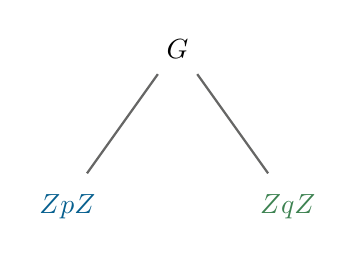
\begin{tikzpicture}
    % (1) Subgroup lines
    \draw[thick, figGray] (-0.25, 1.68) -- (-1.15, 0.42);
    \draw[thick, figGray] (0.25, 1.68) -- (1.15, 0.42);

    % (2) Text nodes last
    \node[inner sep=0.15cm] at (0, 2.0) {$G$};
    \node[inner sep=0.15cm, figBlue] at (-1.4, 0) {$\faktor{\mathbb{Z}}{p\mathbb{Z}}$};
    \node[inner sep=0.15cm, figGreen] at (1.4, 0) {$\faktor{\mathbb{Z}}{q\mathbb{Z}}$};
\end{tikzpicture}
\end{center}

Thus, $G$ always contains copies of $\faktor{\mathbb{Z}}{p\mathbb{Z}}$ and $\faktor{\mathbb{Z}}{q\mathbb{Z}}$; understanding $G$ reduces to understanding how a generator of $\faktor{\mathbb{Z}}{q\mathbb{Z}}$ and a generator of $\faktor{\mathbb{Z}}{p\mathbb{Z}}$ interact.
\end{content}

\begin{speech}[00:31:07 - 00:32:56]
And there's another hint --- this is now for you --- is Sylow $4$, if you think about it, shows that the bigger one, the $\mathbb{Z}$ mod $p\mathbb{Z}$ inside $G$, is normal \inlinemetanote{writes \qt{S IV $\implies$} and \qt{$\faktor{\mathbb{Z}}{p\mathbb{Z}} \subset G$ is Normal}}. This is equivalent to saying that the number of $p$-Sylow subgroups is $1$ \inlinemetanote{writes: (Number of $p$-Sylow subgrps $= 1$)}. Is exactly $1$.

And the way you prove that is you use Sylow $4$ (\cref{thm:sylow-iv}): we know the number is $1$ mod $p$. It's at least $1$. The next chance is $p + 1$, and you show that that's too big --- you can't get to $p + 1$ by the conjugation action.

So, it's normal. That means it's kind of great: we have here $G$, we have $\mathbb{Z}$ mod $p\mathbb{Z}$ in here as a normal subgroup, and we take the generator $x$ here (i.e., in $\faktor{\mathbb{Z}}{q\mathbb{Z}}$) \inlinemetanote{writes \qt{$\faktor{\mathbb{Z}}{p\mathbb{Z}} \subset G$} with \qt{norm.} below it, and adds \qt{$\ni x$} beside $\faktor{\mathbb{Z}}{q\mathbb{Z}}$ in the diagram}. That means $x$ conjugates this \inlinemetanote{gestures from $x$ to $\faktor{\mathbb{Z}}{p\mathbb{Z}}$}.

You know, conjugation by $x$ takes $\mathbb{Z}$ mod $p\mathbb{Z}$ to $\mathbb{Z}$ mod $p\mathbb{Z}$ \inlinemetanote{writes and circles: $\operatorname{Conj}_x \colon \faktor{\mathbb{Z}}{p\mathbb{Z}} \to \faktor{\mathbb{Z}}{p\mathbb{Z}}$}.

And this particular piece of data --- how $x$ acts by conjugation here --- tells you everything about the group, because it tells you the one thing you didn't know: how the generator of $\mathbb{Z}$ mod $q\mathbb{Z}$ and generator of $\mathbb{Z}$ mod $p\mathbb{Z}$ interact.

So, I leave it at that: you can look, there's more you can say here, but you can explore it. If you study what this conjugation could be, you'll classify all possible groups of order $p q$. And it's an interesting thing, and maybe we return to it, but not now. But that's how the stuff that we learned can be used to actually think about these abstract groups. Okay.
\end{speech}

\begin{content}[Normality via Sylow IV and Classification via Conjugation]
Sylow IV (\cref{thm:sylow-iv}) implies that $\faktor{\mathbb{Z}}{p\mathbb{Z}} \subset G$ is a normal subgroup, which is the same as saying that the number of $p$-Sylow subgroups of $G$ is exactly $1$. The lecture leaves this as a hint for the students (\qt{this is now for you}): the number is $1 \bmod p$, so it is $1$ or at least $p + 1$, and $p + 1$ is too big.

\begin{proof}[Proof (beyond the lecture)]
The lecture leaves the details to the students. Let $n_p$ be the number of $p$-Sylow subgroups of $G$. They are all conjugate (\cref{thm:sylow-3}), so they form a single orbit of the conjugation action of $G$, and by the Orbit--Stabilizer Theorem (\cref{thm:orbit-stabilizer}) $n_p$ divides $|G| = pq$. Since $n_p \equiv 1 \pmod p$, $p \nmid n_p$, so $n_p \mid q$. If $n_p \neq 1$, then $n_p \ge p + 1 > q$, which is impossible. Hence, $n_p = 1$. Every conjugate $x A x^{-1}$ of the $p$-Sylow subgroup $A$ is again a $p$-Sylow subgroup, hence equal to $A$, so $A$ is normal in $G$.
\end{proof}

Taking a generator $x \in \faktor{\mathbb{Z}}{q\mathbb{Z}}$, normality of $\faktor{\mathbb{Z}}{p\mathbb{Z}}$ ensures that conjugation by $x$ maps $\faktor{\mathbb{Z}}{p\mathbb{Z}}$ to itself:
\[
\operatorname{Conj}_x \colon \faktor{\mathbb{Z}}{p\mathbb{Z}} \to \faktor{\mathbb{Z}}{p\mathbb{Z}}, \qquad y \mapsto x y x^{-1}.
\]
This map tells how the generators of $\faktor{\mathbb{Z}}{q\mathbb{Z}}$ and $\faktor{\mathbb{Z}}{p\mathbb{Z}}$ interact, and studying what it can be classifies all groups of order $p q$.
\end{content}

\begin{hidden}
% timestamp: 00:32:56
% topic: Classification hints for groups of order p, p^2, and pq
% board_state: ex:order-p2-abelian
% next_goal: Transition to broader directions in group theory (classification, representation theory, Erlangen program / Lie groups)
% open_loops: none
\end{hidden}

\section{Broader Directions in Group Theory}

\begin{speech}[00:33:07 - 00:33:51]
Okay, so, maybe I also say a little bit about group theory in general \inlinemetanote{erases the lower board}.

It's a beginning of many different directions, none of which are represented in this class --- some of which are represented in other classes. But mostly if you want to learn this subject, you have to learn it by yourself. It's somehow too big for classes.
\end{speech}

\subsection{Classification of Finite Simple Groups}

\begin{speech}[00:33:51 - 00:35:02]
Okay, so, maybe I'll just say a few words. We started with this study of $G$, and we mostly considered finite groups \inlinemetanote{writes $G$ on the left with three branching arrows}.

And there's many ways to go forward with this. So, I already mentioned classification \inlinemetanote{writes: Classification}. This classification direction is roughly speaking: if you know, like say, the order of the group, to try to figure out all possible groups of that order. That's the classification problem. It can be reduced to the classification of finite simple groups, so this is usually called the classification of finite simple groups \inlinemetanote{writes: (Classification of finite simple groups)}.

And this is a direction in mathematics that was really exhaustively studied in the $20$th century, so there's an answer to this question, which I don't give now, but roughly speaking there's some infinite families and then there's some exotic elements. So, that's a direction of study. It's maybe not the most active direction now, because that's a full classification.
\end{speech}

\begin{content}[Classification of Finite Simple Groups]
Starting from the study of groups $G$ (mostly finite in this course), a first major direction is \newterm{classification}: determining all groups of a given order. By decomposing finite groups via normal subgroups and quotients, this reduces to the \newterm{classification of finite simple groups}, which was exhaustively studied in the $20$th century: the answer consists of some infinite families and some exotic examples (in textbooks: the sporadic groups).
\end{content}

\subsection{Representation Theory}

\begin{speech}[00:35:02 - 00:35:43]
So, then there's another direction, it's called representation theory \inlinemetanote{writes: Representation theory}.

And this is easy to explain: it basically asks to study homomorphisms from $G$ to matrix groups, $\operatorname{GL}_n$ over some field \inlinemetanote{writes: $( f \colon G \to GL_n(k) )$}. That's the study of such representations, study of homomorphisms \inlinemetanote{writes: study of homoms.}.

And this is an amazingly rich thing to do. Sometimes in Algebra $2$ at the end there's some discussion about this. There's many books on this.
\end{speech}

\begin{content}[Representation Theory]
A second major direction is \newterm{representation theory}: the study of group homomorphisms from $G$ into matrix groups over a field $k$:
\[
\left\{ f \colon G \to \operatorname{GL}_n(k) \right\}.
\]
\end{content}

\subsection{Klein's Erlangen Program and Lie Groups}

\begin{speech}[00:35:43 - 00:37:16]
So, then there's another direction which is maybe the richest vein here, which starts with these ideas of Felix Klein in the $19$th century, and it goes under the name of Klein's Erlangen program \inlinemetanote{writes: F.~Klein (Erlangen Program)}.

Usually, if anything is called a program, it means that that's kind of a slightly propagandistic term and you should be nervous about it... In particular, programs never end, that's just a fact of human politics.

So, this Erlangen program has this really interesting idea. It says that, you know, I motivated groups as you take some geometry and the symmetry is a group, or symmetries of objects are groups. And this Erlangen program has kind of a different perspective: it puts the group in the center. You study groups and their structures, and the geometries then are classified by what their symmetry group is. It's kind of the same thing just said backwards: instead of, you don't start with the geometry and look at the group. Rather, the group is the center thing, and you define geometries by what their symmetry groups are.

That's like Erlangen program in one sentence. Erlangen is a town in southern Germany, it's not so far, I've never been there myself.
\end{speech}

\begin{content}[Klein's Erlangen Program]
A third major direction originates with Felix Klein's \newterm{Erlangen Program} ($19$th century): rather than starting with a geometric space and extracting its symmetry group, one places the group at the center and classifies geometries by their symmetry groups.
\end{content}

\begin{speech}[00:37:16 - 00:38:18]
And one of the most amazing aspects of this --- it was taken seriously by some people --- but Sophus Lie, who's a Norwegian mathematician, he took this very seriously and took an exhaustive study of continuous symmetry groups \inlinemetanote{writes \qt{Sophus Lie} and \qt{$\to$ Study of continuous symmetry groups}}.

Just tried to classify all continuous symmetry groups. And roughly speaking, this is like the two classification worlds: classification of finite simple groups, finite groups --- that's kind of very discrete --- and this is the classification of continuous symmetry groups.

And this has proved to be totally consequential in many directions in $20$th-century mathematics. And so, it's at the center of developments in geometry, topology, and also mathematical physics \inlinemetanote{draws a curved arrow and writes: Center: geometry, topology, math.\ physics}.
\end{speech}

\begin{content}[Sophus Lie and Continuous Symmetry Groups]
Sophus Lie pursued Klein's perspective by systematically classifying \newterm{continuous symmetry groups} (in contrast to the discrete classification of finite simple groups). This theory sits at the center of $20$th-century developments in geometry, topology, and mathematical physics.
\end{content}

\begin{speech}[00:38:18 - 00:40:22]
And the reason for this is that... Well, yeah. So, let me first give you... so the kind of examples that Sophus Lie... And this is also --- this kind of classification theory is complete, you know.

Is how do you find these groups of continuous symmetries? Well, we've seen them already! Like you can take $\operatorname{GL}_n$, let's just say $\mathbb{R}$ \inlinemetanote{writes \qt{$\mathbb{R}^n$} and below it \qt{$GL_n(\mathbb{R})$}}. You can also change the field, but $\operatorname{GL}_n$, that group --- that's a continuous, it's not a finite group, it's kind of continuous symmetries of a vector space. And you could take maybe $\operatorname{SL}_n$, that's the determinant $1$ \inlinemetanote{writes: $SL_n(\mathbb{R})$}. That's just of a vector space $\mathbb{R}^n$.

You could also take a vector space with some kind of inner product and look at the continuous symmetries of that, and these groups are called $O_n$, for the orthogonal groups \inlinemetanote{writes \qt{$\mathbb{R}^n, \langle , \rangle$} and \qt{$O_n$}}. And then you can take $\operatorname{SO}$, that's the... \inlinemetanote{writes: $SO_n$}

Or you could have some complex thing and have a Hermitian inner product, and these things are called the unitary groups and $\operatorname{SU}$ \inlinemetanote{writes \qt{$\mathbb{C}, \langle , \rangle$}, \qt{$U_n$}, and \qt{$SU_n$}}.

Or you could take some kind of vector space --- I don't know if you've learned about this --- but have a symplectic inner product \inlinemetanote{writes: $V, \langle , \rangle^{\text{sympl}}$}. Do you know about that? This is a skew-symmetric inner product. It turns out in that case you have to be even, and this is called the symplectic group \inlinemetanote{writes: $Sp_{2n}$}.

So, these are the standard families of infinite connected groups, and they relate directly to ideas in mathematical physics. For example, this symplectic group turns out to be classical mechanics, and this unitary group is related to quantum mechanics, and this orthogonal group is related to relativity.

And, you know, there's this idea that there's only very few of these continuous symmetry groups. And if you believe that there's some physical equations describing the universe, those equations should be invariant under some continuous group of symmetries of the universe, you are going to inevitably find these groups. And so, that's why they play such an incredibly important role in all of these directions.
\end{speech}

\begin{content}[Overview of Group Theory Directions and Classical Lie Groups]
\definecolor{figBlue}{HTML}{07608F} % RGB (7, 96, 143): petrol blue (MidnightBlue)
\definecolor{figGreen}{HTML}{3D8251} % RGB (61, 130, 81): dark green (ForestGreen!70!black)
\definecolor{figOrange}{HTML}{CC7E2B} % RGB (204, 126, 43): ochre orange (BurntOrange!80!black)
\definecolor{figGray}{HTML}{666665} % RGB (102, 102, 101): dark gray (gray!80!black)
\begin{hidden}
- Canvas: no scale, cm; branching diagram from G on the left to the three main directions, with Lie's branch continuing right
- Boxes: name | lines | w x h (cm) | placed
  G      | 1 letter "$G$" | 0.9 x 0.9 | first, at (0, 0)
  rep    | 2 (\small): "Representation theory" / "$\{f \colon G \to \operatorname{GL}_n(k)\}$" (widest 21 chars = 3.78) | 4.8 x 1.2 | right=1.2cm of G
  cls    | 2 (\small): "Classification" / "(finite simple groups)" (widest 22 chars = 3.96) | 4.8 x 1.2 | above=0.6cm of rep.north west, anchor=south west
  kln    | 1 (\small): "Klein (Erlangen Program)" (24 chars = 4.32) | 5.2 x 0.75 | below=0.6cm of rep.south west, anchor=north west
  lie    | 2 (\small): "Sophus Lie: continuous" / "symmetry groups" (widest 22 chars = 3.96) | 4.8 x 1.2 | right=1.0cm of kln
  ctr    | 3 (\small): "Center:" / "geometry, topology," / "math. physics" (widest 19 chars = 3.42) | 4.2 x 1.65 | above=0.6cm of lie.north, anchor=south
- Width check: G [-0.45, 0.45], gap 1.2 -> boxes start at 1.65; kln reaches 1.65 + 5.2 = 6.85; gap 1.0 -> lie starts at 7.85, reaches 12.65. Total width 13.1 cm <= 14 cm.
- Height check: rep y [-0.6, 0.6]; cls y [1.2, 2.4]; kln y [-1.95, -1.2]; lie y [-2.175, -0.975]; ctr bottom at -0.975 + 0.6 = -0.375, top at 1.275, x in [8.15, 12.35], completely right of rep (ends at 6.45, gap 1.7 cm) and cls (ends at 6.45, gap 1.7 cm).
- Gaps: cls-rep 0.6; rep-kln 0.6; kln-lie 1.0; lie-ctr 0.6; rep-ctr 1.7. All >= 0.5 cm.
- Arrows: G.north east -> cls.west, G.east -> rep.west, G.south east -> kln.west, kln.east -> lie.west, lie.north -> ctr.south.
\end{hidden}
\begin{center}
\begin{tikzpicture}[>=Stealth, font=\small,
  dirbox/.style={draw=figBlue, thick, rounded corners=3pt, fill=figBlue!6, align=center, inner xsep=0.25cm, inner ysep=0.15cm}]
    \node[draw=figGray, thick, circle, minimum size=0.9cm] (G) at (0, 0) {$G$};
    \node[dirbox, minimum width=4.8cm, minimum height=1.2cm, right=1.2cm of G] (rep)
        {Representation theory\\$\{f \colon G \to \operatorname{GL}_n(k)\}$};
    \node[dirbox, minimum width=4.8cm, minimum height=1.2cm, above=0.6cm of rep.north west, anchor=south west] (cls)
        {Classification\\(finite simple groups)};
    \node[dirbox, draw=figGreen, fill=figGreen!6, minimum width=5.2cm, minimum height=0.75cm, below=0.6cm of rep.south west, anchor=north west] (kln)
        {Klein (Erlangen Program)};
    \node[dirbox, draw=figGreen, fill=figGreen!6, minimum width=4.8cm, minimum height=1.2cm, right=1.0cm of kln] (lie)
        {Sophus Lie: continuous\\symmetry groups};
    \node[dirbox, draw=figOrange, fill=figOrange!8, minimum width=4.2cm, minimum height=1.65cm, above=0.6cm of lie.north, anchor=south] (ctr)
        {Center:\\geometry, topology,\\math.\ physics};

    \draw[->, thick, figGray] (G.north east) -- (cls.west);
    \draw[->, thick, figGray] (G.east) -- (rep.west);
    \draw[->, thick, figGray] (G.south east) -- (kln.west);
    \draw[->, thick, figGreen] (kln.east) -- (lie.west);
    \draw[->, thick, figOrange] (lie.north) -- (ctr.south);
\end{tikzpicture}
\end{center}

The classical families of continuous symmetry groups arise as symmetries of vector spaces equipped with geometric structures, and connect directly to physics:
\begin{center}
\begin{tabular}{l l l}
\toprule
\textbf{Underlying Structure} & \textbf{Classical Lie Groups} & \textbf{Physics Connection} \\
\midrule
$\mathbb{R}^n$ (vector space) & $\operatorname{GL}_n(\mathbb{R})$, $\operatorname{SL}_n(\mathbb{R})$ & --- \\
$\mathbb{R}^n, \langle \cdot, \cdot \rangle$ (inner product) & $O_n$, $SO_n$ & Relativity \\
$\mathbb{C}, \langle \cdot, \cdot \rangle$ (Hermitian inner product) & $U_n$, $SU_n$ & Quantum mechanics \\
$V, \langle \cdot, \cdot \rangle^{\text{sympl}}$ (skew-symmetric) & $Sp_{2n}$ & Classical mechanics \\
\bottomrule
\end{tabular}
\end{center}
\end{content}

\begin{hidden}
% timestamp: 00:40:22
% topic: Group theory directions, Erlangen Program, and classical Lie groups
% board_state: classical Lie groups overview
% next_goal: Mention exceptional Lie groups (G_2, F_4, E_6, E_7, E_8) and discuss differential geometry & recent AI/Lean developments
% open_loops: none
\end{hidden}

\begin{speech}[00:40:22 - 00:41:13]
So, there is a class on this, it's usually called like Lie theory or, I don't know, Lie groups \inlinemetanote{writes and boxes: Lie groups}.

And one of the interesting things is that this too has some exotic members. These are the ones that come in families, but it has some exotic members in classification. And these exotic members, I'll just tell you the names of them: there's some $G_2$, $F_4$ --- you know, it's like naming butterflies --- $E_6, E_7, E_8$ \inlinemetanote{writes \qt{$G_2, F_4,$} and \qt{$E_6, E_7, E_8$}}.

And this $E_8$ is really the most exotic, exceptional symmetry group that's classified in this classification, and it's totally a wild structure. It's one of the most beautiful objects in mathematics. It's a group of dimension $248$ \inlinemetanote{draws an arrow from $E_8$ and circles: $248$}.

Anyway, this is the...
\end{speech}

\begin{content}[Exceptional Lie Groups]
Alongside the infinite classical families, the classification of continuous symmetry groups (\newterm{Lie groups}) contains five exceptional (exotic) groups:
\[
G_2, \quad F_4, \quad E_6, \quad E_7, \quad E_8,
\]
where the largest and most intricate, $E_8$, has dimension $248$.
\end{content}

\subsection{Reflections on Lie Groups, Formalization, and AI in Mathematics}

\begin{speech}[00:41:32 - 00:43:31]
But this world of Lie groups is a very different field from the group theory I explain here, because the methods are geometric: they have to do with... all of these groups are manifolds, and the methods of study have to do with differential geometry \inlinemetanote{erases the board}. They sit in the middle of differential geometry and, in some sense, algebra.

Okay. So, we will start the field... I should say that --- and I don't know if you're aware of this --- but this year we're living in may be like the most momentous year in the history of mathematics. I mean, I don't know if you're aware of this, what's going on is amazing.

This has to do with, you know, last week there was this announcement of this Lean proof of Riemann hypothesis, and that's just some kind of amazing advance. The Lean proof is... there's no written proof of Riemann hypothesis, but there's a Lean proof and it's been checked, so it's probably correct, unless you are skeptical about the Lean kernel. Do you think about these things, or not?

And that argument is probably the most intricate, spectacular, complicated argument that humans have ever discovered. It's $17$ million lines of Lean code. Probably before that, like Fermat, when you put that in Lean, it's like $14$ million, but it's kind of maybe comparable in complexity.

So, I mean, it's kind of amazing what's happening, if you follow the applications of these LLMs to mathematics. There was also earlier in the fall this dump of $700$ papers, and there's been some kind of effort to understand, and there's amazing stuff in them.
\end{speech}

\begin{speech}[00:43:31 - 00:45:31]
It's amazing in some sense, and also limited in another sense, which is that it's extremely good at understanding everything and making connections. In terms of the future... I mean, so far it's not good at this kind of developing new theories, new ideas. This is not somehow what it's good at, but what it's amazingly good at is using current known things --- and there's a lot known, you go to the library, it's just full of stuff. It's extremely good at assembling arguments using current known ideas to prove known questions. It's amazingly good at that, and that's totally remarkable. And that only happened this semester!

I would say, in fields I know, that the progress in this semester has kind of been on the order of $5$ or $10$ years of progress, so that's kind of spectacular. And you know, it knows... I've written --- I'm old, I've written a lot of papers --- and it knows my papers better than I do, it's kind of amazing.

Sometimes there'll be an idea, and I remember it's a paper I wrote in the previous century, and of course I remember the theorem --- if the theorem has a lot of hypotheses, you know, I don't remember... they're not all immediately in my head, that's why you write papers. You look at it, and... but it knows all of it, it's amazing.

And one of the things in this $700$ dump was it used some papers that... I mean, there's a lot of papers related to work that I've done, but the one that I found totally remarkable was that there was some work I did on the order of $10$ years ago on a certain theory, and for a certain reason. And it applied that to solve a problem called this Bloch conjecture, which I also knew --- it's kind of an important problem. And the proof is really simple, I mean: it takes these papers I wrote and applies it to this problem, and I knew those papers of course, and I knew the problem.

And if you had asked me, \qt{Could you apply this method to that, to solve that problem?} I would say that it depended on a certain constant, and in our experience --- I wrote those papers with a guy in San Diego, Dragos, a Romanian guy, Dragos --- in our experience when you did this kind of thing you had to compute some coefficient and you mostly got zero. And I would have said you get zero, but actually it's not zero. It's kind of amazing.
\end{speech}

\begin{speech}[00:45:31 - 00:47:26]
So, that's the kind of thing it's amazingly good at, because it has this inexhaustible ability --- like for me to go check that zero takes some time, and I kind of thought it's zero, I mean I was wrong --- but it can just go check it, so it's kind of amazing. That's the kind of... it's amazingly good at that.

And I mean, certainly the math world is changing. How it's going to affect you is a pretty interesting question. I would say that... and I did think this semester, since it's happening this semester, that... And I should say that I'm not... you know, in my group there's some people who are really good at the AI prompting, I don't really prompt so much --- I prompt people, and the people prompt them \inlinemetanote{audience chuckles}.

Yeah, but so for that way it hasn't changed so much for me, but I did think about a class like this: would it make sense to teach it in any different way? And I couldn't --- you know, maybe I don't have enough imagination, but I couldn't think of teaching it in any different way. Meaning that at the level of the material --- this like $19$th-century material --- I don't see how... You know, maybe I say it differently, that before Claude, even last year, everything I say in this class, if you want to learn more or find more, you could just Google it. I mean, in some sense it doesn't change anything from this level: Claude is a more efficient way, because Google, maybe it gives you like three things and you have to pick one that's relevant.

And even before that, there were libraries, and before that there was kind of math friends. So, you know, if you have any \inlinemetanote{audience chuckles}.

So, I don't think somehow a class like this doesn't change --- that we learn here the really basic definitions and results from the $19$th century --- but probably, you know, the idea of what to do as a graduate student will change. Anyway, that's... And I don't know how exactly it changes, but it's definitely an exciting time, man.
\end{speech}

\begin{hidden}
% timestamp: 00:47:26
% topic: Reflections on Lie groups, differential geometry, formalization in Lean, and LLMs in mathematics
% board_state: none (board erased)
% next_goal: Transition after mid-lecture break to Fields and polynomial rings K[x]
% open_loops: none
\end{hidden}

\begin{pause}[Mid-Lecture Break]
The video cuts across the mid-lecture break. When the recording resumes, the projection screen has been lowered, the chalkboards have been erased, and the students are returning to their seats.
\end{pause}

\section{Fields}

\begin{speech}[00:47:27 - 00:48:29]
Okay, so, we start again. And the next topic is about fields \inlinemetanote{writes and underlines: Fields}.

And I already lectured a bit about fields at the beginning of the class. So, when we talked about fields... \inlinemetanote{writes: $k$} The standard letter for a field is $k$, for \emph{Körper}.

When we lectured about fields --- when I lectured about fields at the beginning of the class, we had proven some results, and one of the constructions was to consider this polynomial ring \inlinemetanote{writes: $\rightsquigarrow k[x]$}. That's the polynomials in $x$ \inlinemetanote{writes \qt{poly. in $x$} below $k[x]$}.

So, I hope you remember this object, and we proved some things about it: it's a principal ideal domain, and it's also a unique factorization domain \inlinemetanote{draws an upper arrow from $k[x]$ and writes \qt{PID}, and draws a lower arrow from $k[x]$ and writes \qt{UFD}}. So, that was some ways of studying polynomials whose coefficients are a field.
\end{speech}

\begin{content}[{Recap: The Polynomial Ring \texorpdfstring{$k[x]$}{k[x]}}]
\recap{For a field $k$ (denoted $k$ from the German \emph{Körper}), we previously constructed the polynomial ring $k[x]$ of polynomials in one indeterminate $x$ with coefficients in $k$ (Week 5, \cref{def:poly-ring-k}), and proved that $k[x]$ is both a principal ideal domain ($\mathrm{PID}$, \cref{prop:kx-ideals-principal}) and a unique factorization domain ($\mathrm{UFD}$, Week 6, \cref{ex:kx-ufd}).}

\definecolor{figBlue}{HTML}{07608F} % RGB (7, 96, 143): petrol blue (MidnightBlue)
\definecolor{figGray}{HTML}{666665} % RGB (102, 102, 101): dark gray (gray!80!black)
\begin{hidden}
- Canvas: no scale, cm; small structural map from the board: k -> k[x] (labeled "poly. in x" below) branching to PID and UFD
- Nodes:
  k   at (0, 0)
  kx  at (2.5, 0) holding "$k[x]$" with "poly.\ in $x$" anchored north below it at (2.5, -0.35)
  pid at (4.9, 0.7) anchor west holding "$\mathrm{PID}$"
  ufd at (4.9, -0.7) anchor west holding "$\mathrm{UFD}$"
- Order: (1) arrows k -> kx, kx -> pid, kx -> ufd; (2) text nodes last
- Collisions: pid and ufd are 1.4 cm apart vertically; "poly. in x" sits under kx, left of the branches (starts at x=2.5, branches run to x=4.8).
\end{hidden}
\begin{center}
\begin{tikzpicture}[>=Stealth]
    % (1) Arrows
    \draw[->, thick, figGray, decorate, decoration={snake, amplitude=1.2pt, segment length=6pt, post length=3pt}] (0.4, 0) -- (1.9, 0);
    \draw[->, thick, figBlue] (3.1, 0.1) -- (4.8, 0.65);
    \draw[->, thick, figBlue] (3.1, -0.1) -- (4.8, -0.65);

    % (2) Text last
    \node[inner sep=0.15cm] at (0, 0) {$k$};
    \node[inner sep=0.15cm, figBlue] at (2.5, 0) {$k[x]$};
    \node[anchor=north, inner sep=0.15cm, font=\small, figGray] at (2.5, -0.35) {poly.\ in $x$};
    \node[anchor=west, inner sep=0.15cm, figBlue] at (4.9, 0.7) {$\mathrm{PID}$};
    \node[anchor=west, inner sep=0.15cm, figBlue] at (4.9, -0.7) {$\mathrm{UFD}$};
\end{tikzpicture}
\end{center}
\end{content}

\subsection{Solving Polynomial Equations Over a Field}

\begin{speech}[00:48:29 - 00:49:35]
And we are going to be interested in this second pass at field theory in a different question. It's related to all of this, but a different question. The question, and in some sense a more elementary question: suppose I have a polynomial here --- so this $f$ explicitly has some coefficients, and has a highest degree, because polynomials are finite objects, and it has some lower degrees \inlinemetanote{writes \qt{$f \in k[x]$}, \qt{$f =$}, and \qt{$c_d x^d + c_{d-1} x^{d-1} + \dots + c_0$}}. So, that's like a polynomial.

And the basic problem about polynomials in algebra --- you can't get a more basic problem than this --- is try to solve this polynomial \inlinemetanote{writes and underlines \qt{solve}: Try to solve}. Solve the equation $f(x) = 0$ for... now $x$ is considered some variable \inlinemetanote{writes: $f(x) = 0$}. So, maybe I should put here $\alpha$. The notation is confusing, and it's really... in $k$ \inlinemetanote{overwrites $x$ with $\alpha$ and writes: $f(\alpha) = 0$ for $\alpha \in k$}.

So, we try to solve this polynomial, I mean, we try to find some elements of the field, we stick it in and get zero. That's how you learn to think about polynomials. Try to solve.
\end{speech}

\begin{content}[The Root-Finding Problem]
Given a polynomial $f \in k[x]$ written explicitly in terms of its coefficients as
\[
f = c_d x^d + c_{d-1} x^{d-1} + \dots + c_0 \qquad (c_i \in k),
\]
the fundamental algebraic problem is to solve the polynomial equation:
\[
\text{find } \alpha \in k \quad \text{such that} \quad f(\alpha) = 0.
\]
\end{content}

\begin{speech}[00:49:35 - 00:51:15]
Okay, so, let us think about how to organize that.

So, it could be that if $f$ factors, so that means $f$ is equal to $g_1$ times $g_2$, where these are polynomials \inlinemetanote{writes \qt{If $f$ factors in $k[x]$}, \qt{$f = g_1 \cdot g_2$}, and \qt{poly.} below $g_1 \cdot g_2$}. That has to do with this unique factorization, and we have thought about factorization and we know that some polynomials factor, some don't.

But if we're trying to solve the polynomial and it factors --- so, if $f$ factors, then to solve, meaning find a solution, to solve this $f(\alpha) = 0$, this would be either $g_1(\alpha) = 0$ or $g_2(\alpha) = 0$ \inlinemetanote{draws a large brace and writes \qt{To solve $f(\alpha) = 0$}, \qt{Either $g_1(\alpha) = 0$}, and \qt{or $g_2(\alpha) = 0$}}.

So, this means we can reduce the problem of solving to $g_1$ and $g_2$ \inlinemetanote{writes \qt{$\implies$ Reduce the problem of} and \qt{solving to $g_1, g_2$}}. And of course there's two of them, so that's, you know, the bad part: we only had to consider $f$ to start with and now we have to consider $g_1$ and $g_2$. But they are lower degree. So, it's always better to do this, and these are lower degree \inlinemetanote{writes \qt{lower dgr.} below $g_1, g_2$}. Okay?
\end{speech}

\begin{content}[Reduction via Factorization]
Suppose $f$ factors non-trivially in $k[x]$ as $f = g_1 \cdot g_2$ for polynomials $g_1, g_2 \in k[x]$. Since $k$ is a field (and in particular has no zero divisors), for any $\alpha \in k$ we have:
\[
f(\alpha) = 0 \iff g_1(\alpha) \cdot g_2(\alpha) = 0 \iff \text{either } g_1(\alpha) = 0 \text{ or } g_2(\alpha) = 0.
\]
This reduces the problem of solving $f(\alpha) = 0$ to solving the equations for $g_1$ and $g_2$, each of which has strictly lower degree.
\end{content}

\begin{hidden}
% timestamp: 00:51:15
% topic: Fields: polynomial ring recap and reduction of root-finding via factorization
% board_state: k[x] PID/UFD, root-finding problem f(\alpha)=0, reduction to lower-degree factors
% next_goal: Restrict to irreducible, monic polynomials of degree >= 2
% open_loops: none
\end{hidden}

\begin{speech}[00:51:15 - 00:52:35]
So, this means --- this is a very elementary idea which is, you know, already in any form of high school you went to: if you're trying to solve a polynomial and the polynomial factors, factor it, and try to find a root of one of the factors.

So, this means we should restrict to the case where $f$ is irreducible \inlinemetanote{writes and underlines \qt{irreducible}: This means we should restrict to case where $f$ is irreducible.}. This is using the language of unique factorization: $f$ is irreducible, that means $f$ does not factor. So, the first thing to do, we only think about polynomials which are irreducible, because if they're reducible, we would reduce them and try to solve one of the pieces.

And I remind you this term \qt{irreducible} was technical: this means that $f$ is not zero, $f$ is not a unit, because irreducible polynomials --- we threw these out, you can't be zero or unit \inlinemetanote{writes \qt{$f \neq 0$} and \qt{$f \neq \text{unit}$}}. The units here, by the way, if you remember, the units of $k[x]$ equal the constants that are non-zero \inlinemetanote{writes: $\operatorname{Units}(k[x]) = k^*$}.

So, we don't want --- I mean, this would be silly anyway to try to solve the polynomial zero, that's kind of a waste of time, everything (is a root), and solving a polynomial that's $7$, of course you're not going to find a zero of that. So, these are kind of silly cases.
\end{speech}

\begin{content}[Restriction to Irreducible Polynomials]
By factoring, we restrict attention to the case where $f \in k[x]$ is \newterm{irreducible} (does not factor non-trivially). Recall the technical exclusions in the definition of irreducibility:
\begin{itemize}
    \item $f \neq 0$ (otherwise every $\alpha \in k$ is a trivial solution), and
    \item $f$ is not a unit, where $\operatorname{Units}(k[x]) = k^* = k \setminus \{0\}$ consists of the non-zero constant polynomials (Week 3, \cref{thm:units-polynomial-ring-integral-domain}), which have no roots at all.
\end{itemize}
\end{content}

\begin{speech}[00:52:35 - 00:53:36]
Something else --- so, do you remember this term \qt{irreducible}?

Something else is that we could try to solve a polynomial that's linear, like $c_1 x + c_2$ \inlinemetanote{writes: $f = c_1 x + c_2$}. Then we'd have to solve this: $c_1 \alpha + c_2 = 0$, where these $c_1$ and $c_2$ are in our field \inlinemetanote{writes \qt{$c_1 \alpha + c_2 = 0$} and \qt{$c_1, c_2 \in k$}}. This is also silly, because this is linear algebra \inlinemetanote{writes \qt{lin alg} below $c_1 \alpha + c_2 = 0$}.

We know this, that either it has infinitely many solutions or it has a solution. We're not worried about solving linear polynomials. So, the interesting case --- although it's okay, this is still irreducible \inlinemetanote{adds \qt{irr} above $f = c_1 x + c_2$} --- the interesting case for us will be: case is $f$ is irreducible and the degree of $f$ is at least $2$ \inlinemetanote{writes: Interesting case is: $f$ is irr, and $\operatorname{dg}(f) \ge 2$}.

But this \qt{$f$ is irreducible} in degree $1$ will be contained in the theory, although we just don't have many questions about it, because we know how to solve linear. All right?
\end{speech}

\begin{speech}[00:53:36 - 00:54:37]
So, all of this is saying that, all right, if we're interested in solving, we have this field $k$, I have a polynomial $f \in k[x]$, and I will just start at the beginning that $f$ is irreducible, and usually degree of $f$ is at least $2$ \inlinemetanote{draws vertical divider lines and writes \qt{$k$}, \qt{$f \in k[x]$}, \qt{$f$ is irr.}, and \qt{(usually $\operatorname{dg}(f) \ge 2$)}}. And one more condition, which is very standard, is that $f$ is monic, because, you know, if you're trying to solve the polynomial, you can divide by the leading coefficient and make it monic, it doesn't matter \inlinemetanote{writes: $f$ is monic}. So, these are just kind of standard. If I'm trying to solve... Okay, so...

And it is a fact that you can't always solve. This is a fact that you grow up with, it's some sad fact you learn at some point in your life: you cannot always solve these polynomials.
\end{speech}

\begin{content}[Standard Setup for Root-Finding]
Linear polynomials $f = c_1 x + c_2$ ($c_1, c_2 \in k$, $c_1 \neq 0$) are irreducible, but solving $c_1 \alpha + c_2 = 0$ is immediate ($\alpha = -c_2 / c_1$, linear algebra). Thus, the genuinely interesting case has $\deg(f) \ge 2$. Moreover, dividing by the non-zero leading coefficient does not change the roots, so we may assume $f$ is monic.

Our standard starting data are therefore:
\begin{itemize}
    \item a field $k$,
    \item a polynomial $f \in k[x]$ that is \textbf{irreducible}, \textbf{monic}, and (usually) has $\deg(f) \ge 2$.
\end{itemize}
\end{content}

\subsection{Roots and Linear Factors}

\begin{speech}[00:55:12 - 00:56:32]
All right, so, if you ever find this, here's the first proposition: that if $f$ in $k[x]$ is any polynomial --- so, not all these conditions here --- then there exists $\alpha$ in $k$ such that $\alpha$ is a root if and only if $x - \alpha$ divides $f$ \inlinemetanote{writes \qt{Prop:}, \qt{If $f \in k[x]$ is any poly.}, \qt{then $\exists \alpha \in k$ s.t. $f(\alpha) = 0$}, and \qt{$\iff (x - \alpha) \mid f$}}. Okay?

So, this is something we proved before. This uses --- I'm not going to prove it again --- this uses the division algorithm \inlinemetanote{writes \qt{Div alg for $k[x]$} after a large opening parenthesis}.

Do you remember this argument? Maybe I should write it: you write $f$ is equal to some $g$ times $(x - a)$ --- this is the division algorithm --- plus $f(a)$ \inlinemetanote{writes: $f = g \cdot (x - \alpha) + f(\alpha)$}. When you do the division algorithm here, the remainder is a constant, and that constant has to be $f(a)$. So, if this (i.e., $f(a)$) is zero, is if and only if $x - a$ divides $f$. Okay?
\end{speech}

\begin{content}[Roots and Divisibility by Linear Factors]
\begin{proposition}[Root Factor Characterization]\label[proposition]{prop:root-linear-factor}
If $f \in k[x]$ is any polynomial and $\alpha \in k$, then
\[
f(\alpha) = 0 \iff (x - \alpha) \mid f.
\]
\end{proposition}

\begin{proof}[Proof Sketch (via the Division Algorithm)]
By the division algorithm in $k[x]$ (Week 5, \cref{thm:poly-long-division}), dividing $f$ by the monic degree-$1$ polynomial $(x - \alpha)$ yields a quotient $g \in k[x]$ and a remainder $r \in k[x]$ of degree less than $1$ (hence, a constant $r \in k$):
\[
f = g \cdot (x - \alpha) + r.
\]
Evaluating both sides at $x = \alpha$ gives $f(\alpha) = g(\alpha) \cdot 0 + r = r$, so
\[
f = g \cdot (x - \alpha) + f(\alpha).
\]
Therefore, the remainder $f(\alpha)$ vanishes if and only if $(x - \alpha) \mid f$.
\end{proof}
\end{content}

\begin{speech}[00:56:32 - 00:57:30]
So, the outcome of this is also conceptual: if we ever find something here --- if $f$ is irreducible and degree at least $2$, then there are no solutions \inlinemetanote{writes in brackets: $\bigl[\,\text{If } f \text{ is irr and } \operatorname{dg} \ge 2 \implies \text{There are no solutions!}\,\bigr]$}. Because if there were a solution, I could factor it.

All right? So, the real input is this... The starting point here is we have this $k$, $f \in k[x]$, $f$ irreducible, and if it's degree $2$ or higher, this means there are no solutions \inlinemetanote{draws vertical divider lines and writes \qt{$k$, $f \in k[x]$, $f$ is irr.} and \qt{$\operatorname{dg}(f) \ge 2 \implies \text{No solns in } k$}}.
\end{speech}

\begin{content}[No Roots for Irreducible Polynomials of Degree at Least \texorpdfstring{$2$}{2}]
\begin{corollary}\label[corollary]{cor:irr-deg2-no-roots}
If $f \in k[x]$ is irreducible and $\deg(f) \ge 2$, then $f$ has no solutions (roots) in $k$.
\end{corollary}

\begin{proof}
If there existed $\alpha \in k$ with $f(\alpha) = 0$, then by \cref{prop:root-linear-factor} we could factor $f = g \cdot (x - \alpha)$. Since $\deg(f) \ge 2$, we would have $\deg(g) = \deg(f) - 1 \ge 1$, so neither $g$ nor $(x - \alpha)$ is a unit, contradicting the irreducibility of $f$.
\end{proof}
\end{content}

\begin{hidden}
% timestamp: 00:57:30
% topic: Root-factor characterization and non-existence of roots for irreducible polynomials of degree >= 2
% board_state: prop:root-linear-factor, cor:irr-deg2-no-roots
% next_goal: Give concrete examples (Q, R, F_2) of irreducible polynomials without roots in k, then construct K = k[x]/(f)
% open_loops: none
\end{hidden}

\begin{speech}[00:57:30 - 00:59:04]
And we would like to solve it. So, the examples of this, there's many, and basically all the examples: if you take the field to be $k = \mathbb{Q}$, and I could take the polynomial $f(x)$ is equal to $x^2 - 2$ \inlinemetanote{draws vertical divider lines and writes \qt{$k = \mathbb{Q}$} and \qt{$f(x) = x^2 - 2$}}. This has no solution in $\mathbb{Q}$ because you cannot find a square root of $2$ in $\mathbb{Q}$.

Or you could take this $k$ to be $\mathbb{R}$, and you take $f(x)$ is equal to $x^2 + 1$ \inlinemetanote{writes \qt{$k = \mathbb{R}$} and \qt{$f(x) = x^2 + 1$}}. Also no solution.

Or you could take $k$ is equal to the field $\mathbb{F}_2$, and I think this polynomial \inlinemetanote{writes \qt{$k = \mathbb{F}_2$} and \qt{$f(x) = x^2 + x + 1$}}. We take this polynomial, we can just try: does this have a solution? Well, there's only two elements of $\mathbb{F}_2$, so it's not going to take a long time to check. If we put in $f(0)$, that's $1$, and $f(1)$, well that's also $1$ \inlinemetanote{writes \qt{$f(0) = 1$} and \qt{$f(1) = 1$} inside a bracket}. So, this is correct.

These are all examples where you take a field, you take some polynomial --- the interesting case is degree at least $2$ --- and then if it's irreducible, it will not have a solution, or these ones don't have solutions. Anyway, the beginning of this discussion is you have this field, you have a polynomial which we'll take to be irreducible, and we would like to solve it. Although we can't solve it. So, what can we do here?
\end{speech}

\begin{content}[Examples of Irreducible Polynomials Without Roots]
\begin{examples}\label[examples]{exm:irreducible-no-roots}
Each of the following degree-$2$ polynomials has no root in its base field $k$ (and since its degree is $2$, having no root implies it is irreducible over $k$):
\begin{enumerate}[label=\textbf{\arabic*.}]
    \item $k = \mathbb{Q}$, $f(x) = x^2 - 2$: has no solution in $\mathbb{Q}$ since $\sqrt{2} \notin \mathbb{Q}$.
    \item $k = \mathbb{R}$, $f(x) = x^2 + 1$: has no solution in $\mathbb{R}$ since $\alpha^2 + 1 \ge 1 > 0$ for all $\alpha \in \mathbb{R}$.
    \item $k = \mathbb{F}_2$, $f(x) = x^2 + x + 1$: checking all elements of $\mathbb{F}_2 = \{0, 1\}$ directly gives:
    \[
    f(0) = 0^2 + 0 + 1 = 1 \neq 0, \qquad f(1) = 1^2 + 1 + 1 = 1 \neq 0.
    \]
\end{enumerate}
\end{examples}

\begin{steps}[Why No Roots Implies Irreducibility in Degree \texorpdfstring{$2$}{2} or \texorpdfstring{$3$}{3}]
Going beyond the lecture: if a polynomial $f \in k[x]$ of degree $2$ or $3$ factored non-trivially as $f = g_1 \cdot g_2$ with $\deg(g_1), \deg(g_2) \ge 1$, then at least one factor would have degree $1$, giving a root in $k$ by \cref{prop:root-linear-factor}. Thus, in degrees $2$ and $3$, having no roots in $k$ is equivalent to being irreducible over $k$.
\end{steps}
\end{content}

\begin{speech}[00:59:04 - 01:00:02]
\inlinemetanote{erases the lower board} So, yeah, I'd say this discussion in a sense is really closer to the spirit of high school algebra: you know, you try to actually solve polynomials.
\end{speech}

\subsection{Constructing a Field Extension \texorpdfstring{$K = \faktor{k[x]}{(f)}$}{K = k[x]/(f)}}

\begin{speech}[01:00:02 - 01:01:34]
So, yeah, the starting point, which I've said now many times, here we have this $k$ \inlinemetanote{writes: $k$}. You imagine you have this $k$, and you have this particular polynomial here, and $f$ is irreducible \inlinemetanote{writes \qt{$f \in k[x]$} and \qt{$f$ is irr.}}.

And as I said, this leaves the possibility logically that $f$ is a linear polynomial, and it's okay. You usually don't have any problem with that.

Then you say --- and you want to solve it, and you say you can't solve it --- you can wish: \qt{I wish I could solve this polynomial equation} \inlinemetanote{writes: I wish I could solve this poly.\ equation.}.

You can wish. And, you know, \qt{in dreams begin responsibilities}. So, now maybe this could be called wish $1$ \inlinemetanote{writes and underlines above: Wish 1:}.

If you... maybe you're lucky now and a genie comes. I once looked up the word for genie in German some years ago, and the one I liked the best is \emph{Wunschgeist}. The Germans somehow have a super direct language.

And one thing about genies you know that they always give you three wishes. And the reason is because of the human weakness for desiring things that are very close. That's kind of an expression of that --- the reason genies give you three wishes is because of that weakness, and we're going to see it here.
\end{speech}

\begin{speech}[01:01:34 - 01:02:36]
So, wish $1$, I want this, and so this is the granting of this wish: we make a field $K$ \inlinemetanote{writes and underlines \qt{Granting 1:} and writes \qt{$K$}}.

This is very standard notation, and for this my board work has to be good, because I will try to keep that there will be this little $k$, that's the field we start with, and the big $K$ is the field that is granted by the genie.

So, it's this field, and as you'll see, the genie writes down this field: $K = \faktor{k[x]}{(f)}$ \inlinemetanote{writes: $= \faktor{k[x]}{(f)}$}.

So, what is this object? This is a ring, and that's an ideal \inlinemetanote{draws an upper arrow from $k[x]$ and writes \qt{ring}, and draws a lower arrow from $(f)$ and writes \qt{ideal}}. That's the ideal generated by $f$. All right? You should grant me that this thing exists: it's a quotient, it's a ring quotient by an ideal, so this is some ring \inlinemetanote{underlines $K = \faktor{k[x]}{(f)}$ and writes \qt{Ring} below}. This is a ring.
\end{speech}

\begin{content}[{Granting Wish 1: The Quotient Ring \texorpdfstring{$K := \faktor{k[x]}{(f)}$}{K := k[x]/(f)}}]
Starting from a base field $k$ and an irreducible polynomial $f \in k[x]$ (which in general has no root in $k$), we construct a larger algebraic structure by forming the quotient ring:
\[
K := \faktor{k[x]}{(f)},
\]
where $k[x]$ is the polynomial ring and $(f) := f \cdot k[x]$ is the principal ideal generated by $f$. Note the notation convention: lowercase $k$ denotes the original base field, while uppercase $K$ denotes the constructed quotient object.
\end{content}

\begin{insight}[The Genie (\emph{Wunschgeist}) and the Three Wishes]
The lecturer frames the construction of field extensions through a playful analogy: we wish to solve an irreducible polynomial $f \in k[x]$ (\qt{Wish 1}). As the lecturer quotes (\qt{in dreams begin responsibilities}), the \emph{Wunschgeist} grants this wish by handing us the quotient ring $K = \faktor{k[x]}{(f)}$ --- and, as with classic genie tales of three wishes, solving one equation naturally leads to further wishes.
\end{insight}

\begin{speech}[01:02:36 - 01:03:42]
Okay, so, the first claim is that $K$ is a field \inlinemetanote{writes: (1) $K$ is a field}.

All right, let's try to prove this. Proof: $K$ is a field, this big $K$ is a field, if and only if this ideal is a maximal ideal \inlinemetanote{writes \qt{proof}, \qt{$K$ is a field}, and \qt{$\iff (f)$ is a max.\ ideal}}.

So, the issue here you have to remember now things back to the beginning of the class. If you have a ring quotient by an ideal, the only way this can be a field is if it's a maximal ideal, and if it's a maximal ideal, it's a field. So, we have to check that $(f)$ inside $k[x]$ is a maximal ideal \inlinemetanote{writes: We have to check that $(f) \subset k[x]$ is a max.\ ideal.}.

Then you have to remember: what is a maximal ideal? A maximal ideal is an ideal such that if I try... so first of all, let's check this slowly because it's been a long time.
\end{speech}

\begin{content}
\begin{claim}[\texorpdfstring{$K = \faktor{k[x]}{(f)}$}{K = k[x]/(f)} is a Field]\label[claim]{clm:quotient-is-field}
For any field $k$ and any irreducible polynomial $f \in k[x]$, the quotient ring $K = \faktor{k[x]}{(f)}$ is a field.
\end{claim}
\end{content}

\begin{proofWrapper}[Proof of \cref{clm:quotient-is-field}]

\begin{hidden}
% timestamp: 01:04:39
% topic: Constructing K = k[x]/(f) and proving it is a field via maximal ideals
% board_state: clm:quotient-is-field
% next_goal: Prove (f) is a maximal ideal in k[x] using the PID property and irreducibility of f
% open_loops: none
\end{hidden}

\begin{speech}[01:04:39 - 01:05:54]
Okay, just to remind you because it's been a long time.

The first thing is that to be a maximal ideal, $(f)$ can't be all of the thing \inlinemetanote{writes \qt{To be a max ideal:} (underlined) and \qt{$(f) \neq k[x]$}}. Maximal ideals are not the whole --- that's part of the definition, right? And this is true by definition since $f$ is not a unit \inlinemetanote{writes: True by def since $f \neq$ unit}. Irreducible implies it's not a unit. All right? I mean, the only way this would be true is if $f$ were a constant polynomial, and we're ruling that out.

The second thing we have to show is that suppose I have an ideal in between, then either $I$ is equal to $(f)$ or $I$ is equal to the whole thing \inlinemetanote{writes \qt{Suppose $(f) \subset I \subset k[x]$} and \qt{then either $I = (f)$ or $I = k[x]$}}.

Those are the two conditions to be a maximal ideal. Do you remember this? That means the ideal's a champion: you cannot beat it without being the whole, right?
\end{speech}

\begin{content}[Maximal Ideal Criterion and Properness]
Recall that for a ring $R$ and an ideal $m \subset R$, the quotient $\faktor{R}{m}$ is a field if and only if $m$ is a maximal ideal (Week 5, \cref{prop:quotient-field-maximal}). Thus, it suffices to verify that $(f) \subset k[x]$ is a maximal ideal, which requires two conditions:

\textbf{Condition 1 (Proper ideal):} $(f) \neq k[x]$.
Indeed, $1 \in (f)$ would mean $1 = f \cdot q$ for some $q \in k[x]$, making $f$ a unit. Since $f$ is irreducible, $f$ is not a unit by definition, so $(f) \neq k[x]$.

\textbf{Condition 2 (Maximality):} Whenever $I \subset k[x]$ is an ideal with $(f) \subset I \subset k[x]$, either $I = (f)$ or $I = k[x]$.
\end{content}

\begin{speech}[01:05:54 - 01:08:17]
So, how do we prove this? We need to prove this, so suppose $(f) \subset I \subset k[x]$ \inlinemetanote{writes: Suppose $(f) \subset I \subset k[x]$}.

But what we know: since $k[x]$ is a $\mathrm{PID}$, this implies that $I$ is actually generated by one element, because it's a principal ideal domain \inlinemetanote{writes \qt{Since $k[x]$ is a PID} and \qt{$\implies I = (g)$}}.

This would mean that $(f)$ is inside $(g)$, and then this would mean that $g$ divides $f$ \inlinemetanote{writes \qt{$\implies (f) \subset (g)$} and \qt{$g \mid f$}}. That's what it means, because $f$ is an element of things that are multiples of $g$. In particular, it means $f$ is equal to $g$ times somebody \inlinemetanote{writes: $f = g \cdot h$}. All right? That's what it means for $g$ to divide $f$.

Now we use the fact $f$ is irreducible \inlinemetanote{writes: $f$ is irr}. If you remember what irreducible means: if you have an irreducible element and you try to factor it, then one of these things has to be a unit. Means either $g$ or $h$ is a unit \inlinemetanote{writes: $\implies$ either $g$ or $h$ is a unit.}. That's the definition of irreducible.

If $g$ is a unit, then this ideal is the whole ring \inlinemetanote{writes: $g$ is unit $\implies I = k[x]$}. So, that's not possible (meaning that gives the second alternative) because we have it here. If $h$ is a unit, then the ideal is equal to $(f)$, so: $g$ is a unit implies $I$ is equal to $k[x]$; $h$ is a unit implies $(f)$ is equal to $(g)$ \inlinemetanote{writes: $h$ is unit $\implies (f) = (g)$}.

So, we've proven that if we try to find an ideal bigger, then it either has to be this one or that one. That shows it's maximal. All right.
\end{speech}

\begin{content}[Verifying Maximality via the PID Property]
Suppose $I \subset k[x]$ is an ideal satisfying $(f) \subset I \subset k[x]$. Since $k[x]$ is a $\mathrm{PID}$, every ideal is principal, so there exists $g \in k[x]$ such that
\[
I = (g).
\]
From $(f) \subset (g)$, we have $f \in (g)$, which means $g \mid f$, so there exists $h \in k[x]$ such that
\[
f = g \cdot h.
\]
Since $f$ is irreducible, by definition either $g$ or $h$ must be a unit in $k[x]$:
\begin{itemize}
    \item If $g$ is a unit, then $1 = g \cdot g^{-1} \in (g) = I$, so $I = k[x]$.
    \item If $h$ is a unit, then $g = f \cdot h^{-1} \in (f)$, so $(g) \subset (f)$, and hence $I = (g) = (f)$.
\end{itemize}
Therefore, $(f)$ is a maximal ideal of $k[x]$, and consequently $K = \faktor{k[x]}{(f)}$ is a field.
\end{content}

\end{proofWrapper}

\begin{speech}[01:08:17 - 01:09:07]
The first step is to understand for this granting of the wish that this $\faktor{k[x]}{(f)}$ is a field. It's born a ring, but since it's maximal, it's a field. So, that's one.

Okay. The second thing --- see, it's all going to be very simple and almost tautological, and you're going to regret you made this wish \inlinemetanote{erases the lower chalkboard}.

The first statement was $K$ is a field. Maybe I leave that up here.
\end{speech}

\begin{hidden}
% timestamp: 01:09:10
% topic: Completed proof that K = k[x]/(f) is a field; starting canonical embedding k subset K
% board_state: clm:quotient-is-field (proved)
% next_goal: Define and prove canonical embedding k -> K
% open_loops: none
\end{hidden}

\begin{speech}[01:09:07 - 01:11:18]
I write it in the corner: so, $K = \faktor{k[x]}{(f)}$ is a field \inlinemetanote{writes: $K = \faktor{k[x]}{(f)}$ is a field}. So, we've proven that \inlinemetanote{draws a checkmark beside \qt{is a field}}.

The second is that our original $k$ sits inside $K$ canonically \inlinemetanote{writes: $k \subset K$ canonically}. This is a difficult subject if you have bad handwriting, all right? So, my big $K$ is a field, we've proven it, and the second is that the little $k$ we started with sits inside canonically. It's a subfield.

And the proof of this is just I give you the map: if you have an element, say $\gamma$ in little $k$, how do I get to big $K$? I just consider the quotient class of $\gamma$ in big $K$ \inlinemetanote{writes \qt{pf: $\gamma \in k$} and \qt{$\longmapsto \bar{\gamma} \in K$}}. And that's the homomorphism from little $k$ to big $K$ \inlinemetanote{writes: $\Phi \colon k \to K$}. It's just you take the equivalence class, and nothing else happens.

So, you have to worry: this is a homomorphism from one field to the other. So, there are only two possibilities: either it's an injection, or it's zero --- but it can't be zero because $1$ goes to $1$. Another way to say it is that if I take two constants... how could a constant that's not zero go to zero here? The only way is if that constant were in this ideal. But that's impossible, because this is some polynomial of some degree; this ideal doesn't have any constants in it. So, the constants live.

This is a confusing way of saying something very simple: this quotient has the notion of the little field in it by taking the constants here, and they never die because a constant can't be a multiple of $f$. So, it's a little confusing, but actually nothing's gone on here.
\end{speech}

\begin{content}[{Canonical Embedding of \texorpdfstring{$k$}{k} into \texorpdfstring{$K$}{K}}]
\begin{claim}[\texorpdfstring{$k \subset K$}{k subset K} Canonically]\label[claim]{clm:canonical-embedding}
The original field $k$ sits canonically inside $K = \faktor{k[x]}{(f)}$ as a subfield.
\end{claim}

\begin{proof}
Define the map $\Phi \colon k \to K$ by sending each element $\gamma \in k$ (viewed as a constant polynomial in $k[x]$) to its residue class modulo $(f)$:
\[
\gamma \in k \longmapsto \bar{\gamma} \in K.
\]
This map is a ring homomorphism between two fields sending $1_k$ to $\bar{1}_K$. A ring homomorphism out of a field is either injective or identically zero; since $1_k \mapsto \bar{1} \neq \bar{0}$ (as $\deg(f) \ge 1$, the ideal $(f)$ contains no non-zero constants), the kernel is $\{0\}$. Equivalently, no non-zero constant $\gamma \in k$ can be a multiple of $f$. Thus, $\Phi$ is injective, embedding $k$ canonically as a subfield of $K$.
\end{proof}

\begin{steps}[Why the Ideal \texorpdfstring{$(f)$}{(f)} Contains No Non-Zero Constants]
Any non-zero element of the principal ideal $(f)$ has the form $f \cdot q$ with $q \neq 0$ in $k[x]$, so its degree is $\deg(f) + \deg(q) \ge \deg(f) \ge 1$ (since $f$ is irreducible and hence not a unit). Therefore, $(f) \cap k = \{0\}$, so distinct constants in $k$ remain distinct modulo $(f)$.
\end{steps}
\end{content}

\subsubsection{Field Extensions and Existence of a Root in \texorpdfstring{$K$}{K}}

\begin{speech}[01:11:18 - 01:13:26]
Right, so, what we have is what's called a \newterm{field extension}. We have our little $k$, and it sits inside big $K$ \inlinemetanote{writes \qt{$k$} and writes \qt{$K$} above $k$ connected by a vertical line}. Often it's written like this. If you see this in a math book, this is called a field extension, and it just means you have one field inside another field \inlinemetanote{writes \qt{field extension} with an arrow pointing to the diagram, and writes \qt{$k \subset K$}}. That's all it means. And here, there's this identification: this field exists by itself, and we put it inside by taking the equivalence classes. All right.

So, that's step two. The answer to the question: first is this production of the big field $K$, and the second is realizing our little field lives inside the big field, and of course the third is the root, the production of the root \inlinemetanote{writes: Root:}. And so, we let $\alpha$ in big $K$ be the equivalence class of $x$ \inlinemetanote{writes \qt{$\alpha \in K$} and \qt{$\alpha = \bar{x}$}}. Okay?

Now I've given you, or the genie's given you, this big field, this is the original field that you were suffering with, and also an element \inlinemetanote{writes \qt{$K$}, \qt{$k$} below $K$ connected by a vertical line, and \qt{$\ni \alpha$}}. Do you agree? And almost nothing's happened here. But do you agree with this? It's important to understand: this is $\bar{x}$, and $\bar{x}$ is a well-defined element here (i.e., in $K$), meaning it's the equivalence class of $x$.

All right. And now the third thing is we check: we take this polynomial; the polynomial was born here, little $k$ \inlinemetanote{writes: $f \in k[x]$}. But we can also view it --- since this is inside big $K$ --- we can view this polynomial to be a polynomial here, because little $k$ are just some elements of big $K$, so we can just view it as a polynomial with coefficients in big $K$ \inlinemetanote{writes \qt{$\subset K[x]$}, \qt{we can view}, and \qt{$f \in K[x]$}}.
\end{speech}

\begin{content}[Field Extensions and the Element \texorpdfstring{$\alpha = \bar{x} \in K$}{alpha = x-bar in K}]
\begin{definition}[Field Extension]\label[definition]{def:field-extension}
When a field $k$ is a subfield of a field $K$ ($k \subset K$), we call $K$ a \newterm{field extension} of $k$ (often depicted as a vertical tower with $K$ above $k$).
\end{definition}

Using the canonical embedding $k \subset K$ from \cref{clm:canonical-embedding}, we define the candidate root $\alpha \in K$ as the residue class of the indeterminate $x$:
\[
\alpha := \bar{x} \in K = \faktor{k[x]}{(f)}.
\]
Moreover, because $k \subset K$, any polynomial $f \in k[x]$ can be viewed as a polynomial with coefficients in $K$, i.e., $f \in k[x] \subset K[x]$.

\definecolor{figBlue}{HTML}{07608F} % RGB (7, 96, 143): petrol blue (MidnightBlue)
\definecolor{figRed}{HTML}{B5251C} % RGB (181, 37, 28): brick red (BrickRed)
\definecolor{figGray}{HTML}{666665} % RGB (102, 102, 101): dark gray (gray!80!black)
\begin{hidden}
- Canvas: no scale, cm; two small board diagrams side by side: left shows field extension tower K over k with "field extension" label; right shows K \ni \alpha over k
- Order: (1) vertical tower segments and pointer arrow; (2) all text last
- Coordinates:
  Left panel: K at (0, 1.8), k at (0, 0); vertical line from (0, 0.35) to (0, 1.45); note "field extension" at (1.3, 1.35) with thin arrow to (0.15, 0.95); "k \subset K" at (0, -0.75)
  Right panel (x shifted by 6.0): K at (6.0, 1.8) and "\ni \alpha = \bar{x}" anchor west at (6.35, 1.8), k at (6.0, 0); vertical line from (6.0, 0.35) to (6.0, 1.45)
- Collisions: left panel x in [-0.4, 4.0], right panel starts at x = 5.65, gap >= 1.65 cm; "\ni \alpha = \bar{x}" starts at 6.35, clear of K.
\end{hidden}
\begin{center}
\begin{tikzpicture}[>=Stealth]
    % (1) Lines and arrow
    \draw[thick, figGray] (0, 0.35) -- (0, 1.45);
    \draw[->, thin, figBlue] (1.3, 1.35) -- (0.15, 0.95);
    \draw[thick, figGray] (6.0, 0.35) -- (6.0, 1.45);

    % (2) Text last
    \node[inner sep=0.15cm, figBlue] at (0, 1.8) {$K$};
    \node[inner sep=0.15cm] at (0, 0) {$k$};
    \node[anchor=west, inner sep=0.15cm, figBlue, font=\small] at (1.3, 1.35) {field extension};
    \node[inner sep=0.15cm] at (0, -0.75) {$k \subset K$};

    \node[inner sep=0.15cm, figBlue] at (6.0, 1.8) {$K$};
    \node[anchor=west, inner sep=0.15cm, figRed] at (6.35, 1.8) {$\ni \alpha = \bar{x}$};
    \node[inner sep=0.15cm] at (6.0, 0) {$k$};
\end{tikzpicture}
\end{center}
\end{content}

\begin{hidden}
% timestamp: 01:13:26
% topic: Canonical embedding k subset K, field extensions, and defining alpha = x-bar in K
% board_state: clm:canonical-embedding, def:field-extension
% next_goal: Verify f(alpha) = 0 in K, summarize Wish 1, and present R[x]/(x^2+1) \cong C
% open_loops: none
\end{hidden}

\begin{speech}[01:13:26 - 01:15:23]
And the last thing to check, which is not a surprise, is that $\alpha$ solves the polynomial \inlinemetanote{swaps the lower board up and the upper board down, and erases the lower board}.

So, the first claim was that big $K$ is a field, the second claim is that little $k$ sits naturally inside it, then we produced this element $\alpha$, and the third claim is that if I take $f$ of $\alpha$, this equals zero in big $K$ \inlinemetanote{writes: $f(\alpha) = 0$ in $K$}.

First I'd like to see it makes sense, because said $f$ is this polynomial --- it makes sense: $\alpha$ is an element of $K$, I can stick $\alpha$ in there, I get some number. The claim is I get zero.

So, the proof of this is that, okay, let's try to do it: $f$ of $\alpha$, well, this is $f$ of $\bar{x}$, because $\alpha$ is $\bar{x}$ \inlinemetanote{writes \qt{pf:}, \qt{$f(\alpha) =$}, and \qt{$f(\bar{x})$}}. $f$, all its coefficients are just elements of little $k$, so this is equal to $\overline{f}$ \inlinemetanote{writes: $= \overline{f(x)}$}. And $\overline{f}$ is equal to zero in $\faktor{k[x]}{(f)}$, precisely because we're taking out $f$, which equals $K$ \inlinemetanote{writes \qt{$= 0$}, \qt{$\in \faktor{k[x]}{(f)}$}, and \qt{$= K$} and draws a QED box}. So, that's the end of it.

Right? It's entirely tautological, this construction.
\end{speech}

\begin{content}[Verification that \texorpdfstring{$f(\alpha) = 0$}{f(alpha) = 0} in \texorpdfstring{$K$}{K}]
\begin{claim}[\texorpdfstring{$\alpha$}{alpha} is a Root of \texorpdfstring{$f$}{f} in \texorpdfstring{$K$}{K}]\label[claim]{clm:alpha-is-root}
With $\alpha := \bar{x} \in K$, we have $f(\alpha) = 0$ in $K$.
\end{claim}

\begin{proof}
Viewing $f \in k[x] \subset K[x]$, we evaluate $f$ at $\alpha = \bar{x} \in K$:
\[
f(\alpha) = f(\bar{x}) = \overline{f(x)} = 0 \in \faktor{k[x]}{(f)} = K,
\]
since $f(x) \in (f)$ represents the zero residue class in the quotient $\faktor{k[x]}{(f)}$.
\end{proof}

\begin{steps}[Expanding the Quotient Evaluation Explicitly]
Writing $f(x) = c_d x^d + c_{d-1} x^{d-1} + \dots + c_0$ with $c_i \in k$, the canonical embedding identifies each coefficient $c_i$ with $\bar{c}_i \in K$. Because addition and multiplication in the quotient ring $\faktor{k[x]}{(f)}$ satisfy $\bar{a} + \bar{b} = \overline{a + b}$ and $\bar{a} \cdot \bar{b} = \overline{a \cdot b}$, we have:
\begin{align*}
f(\alpha) &= \bar{c}_d \bar{x}^d + \bar{c}_{d-1} \bar{x}^{d-1} + \dots + \bar{c}_0 \\
&= \overline{c_d x^d + c_{d-1} x^{d-1} + \dots + c_0} \\
&= \overline{f(x)} = \bar{0} \in K.
\end{align*}
\end{steps}
\end{content}

\begin{speech}[01:15:23 - 01:17:00]
So, that's the answer to the wish here: you start with this $k$, and $f$ in $k$ of $x$ irreducible, and you wish for a solution, and the granting of this wish is this field extension --- you have to go to a bigger field, because we know there's no solutions in that field --- a field extension and an element such that you can solve \inlinemetanote{writes \qt{$k, \; f \in k[x]$ irr}, draws a downward double arrow, and writes \qt{$K$} over \qt{$k$} connected by a vertical line, \qt{$\ni \alpha$}, and \qt{s.t.\ $f(\alpha) = 0$}}.

That's the specific granting of the wish. And everything here is explicit: this thing is that, and this is $\bar{x}$, okay \inlinemetanote{writes \qt{$\faktor{k[x]}{(f)} = K$} and \qt{$\bar{x} = \alpha$}}? It's totally explicit, maybe completely unsatisfying, because the whole matter is tautological, but this is a really important construction. Are there any questions about it?

I mean, it's really the basis of many different ideas, but it says that if you have this field, the little $k$, and you find an irreducible polynomial, one thing is to feel sad you cannot solve that polynomial. The other side of the coin is that polynomial is creating you a beautiful new field, this one \inlinemetanote{points at $\faktor{k[x]}{(f)} = K$}. And this field is maybe one you didn't know before; it's giving you a new field, and moreover it's giving you a solution for that polynomial in that field.
\end{speech}

\begin{content}[Summary of Wish 1 Granted]
\definecolor{figBlue}{HTML}{07608F} % RGB (7, 96, 143): petrol blue (MidnightBlue)
\definecolor{figRed}{HTML}{B5251C} % RGB (181, 37, 28): brick red (BrickRed)
\definecolor{figGray}{HTML}{666665} % RGB (102, 102, 101): dark gray (gray!80!black)
\begin{hidden}
- Canvas: no scale, cm; summary flow from initial data (k, f in k[x] irr) down to granted extension K ni alpha over k with f(alpha)=0, and explicit identifications on the left
- Order: (1) downward arrow from top data to K; (2) vertical line K--k; (3) all text last
- Coordinates:
  Top: "(0, 2.95)" holding "$k, \; f \in k[x] \text{ irr}$"
  Downward double arrow (the board has a double arrow, not a squiggle) from (0, 2.55) to (0, 1.7)
  Tower: K at (0, 1.3), k at (0, 0), vertical line (0, 0.32) to (0, 0.98)
  Left annotations: "\faktor{k[x]}{(f)} =" anchor east at (-0.45, 1.3)
  Right annotations: "\ni \alpha" anchor west at (0.3, 1.3), "\bar{x} = \alpha" anchor west at (0.4, 1.9), "s.t.\ f(\alpha) = 0" anchor west at (0.55, 0.65)
- Collisions: vertical tower at x=0; left formula ends at -0.45; right labels start at +0.3 and are stacked at distinct y values (1.9, 1.3, 0.65).
\end{hidden}
\begin{center}
\begin{tikzpicture}[>=Stealth]
    % (1), (2) Construction arrow and tower line
    \draw[-{Implies}, double, thick, figBlue] (0, 2.55) -- (0, 1.7);
    \draw[thick, figGray] (0, 0.32) -- (0, 0.98);

    % (3) Text last
    \node[inner sep=0.15cm] at (0, 2.95) {$k, \; f \in k[x] \text{ irr}$};
    \node[inner sep=0.15cm, figBlue] at (0, 1.3) {$K$};
    \node[inner sep=0.15cm] at (0, 0) {$k$};
    \node[anchor=east, inner sep=0.15cm, figBlue] at (-0.45, 1.3) {$\faktor{k[x]}{(f)} =$};
    \node[anchor=west, inner sep=0.15cm, figRed] at (0.3, 1.3) {$\ni \alpha$};
    \node[anchor=west, inner sep=0.15cm, figRed] at (0.4, 1.9) {$\bar{x} = \alpha$};
    \node[anchor=west, inner sep=0.15cm] at (0.55, 0.65) {s.t.\ $f(\alpha) = 0$};
\end{tikzpicture}
\end{center}

Everything in this construction is completely explicit: $K = \faktor{k[x]}{(f)}$ is a field containing $k$ canonically, and $\alpha = \bar{x} \in K$ satisfies $f(\alpha) = 0$.
\end{content}

\begin{speech}[01:17:00 - 01:18:26]
So, for example, if you do this with $\mathbb{R}$ --- the most famous example is if your little field is $\mathbb{R}$, and your polynomial is $x^2 + 1$ --- then what this construction gives you is $\mathbb{R}$ adjoin $x$ modulo $x^2 + 1$ \inlinemetanote{writes \qt{$k = \mathbb{R}$}, \qt{$f = x^2 + 1$}, and \qt{$K = \faktor{\mathbb{R}[x]}{(x^2+1)}$}}.

And it was an exercise, or we discussed, this is isomorphic actually to the complex numbers \inlinemetanote{writes: $\cong \mathbb{C}$}. And the isomorphism takes $\bar{x}$ to $i$, and so that $\alpha$ is $i$ \inlinemetanote{writes \qt{$\alpha = \bar{x} = i$} and draws $K$ over $\mathbb{R}$}. It gives you the complex numbers. If you understood all of this before discovering the complex numbers --- I think no human has done that, but anyway --- if you developed algebra up to here without discovering the complex numbers, and you said, \qt{Okay, I'll start with $\mathbb{R}$, and this is the polynomial I want to find,} you get the complex numbers.

And you get lots and lots of other fields. This is a spectacularly rich way to make fields: you take any field you want, and you take any polynomial you can't solve that's irreducible, and then you get a new field. All right.
\end{speech}

\begin{content}
\begin{example}[Constructing \texorpdfstring{$\mathbb{C}$}{C} from \texorpdfstring{$\mathbb{R}$}{R} and \texorpdfstring{$x^2 + 1$}{x\textasciicircum 2 + 1}]\label[example]{ex:complex-numbers-quotient}
Take $k = \mathbb{R}$ and the irreducible polynomial $f(x) = x^2 + 1 \in \mathbb{R}[x]$. The quotient construction produces the field extension
\[
K = \faktor{\mathbb{R}[x]}{(x^2 + 1)} \cong \mathbb{C},
\]
where the isomorphism sends the canonical root $\alpha = \bar{x} \in K$ to the imaginary unit $i \in \mathbb{C}$ (satisfying $i^2 + 1 = 0$). Week 4 proved the same over $\mathbb{Q}$: $\faktor{\mathbb{Q}[x]}{(x^2+1)} \cong \mathbb{Q}[i]$ (\cref{thm:first-isom-applied-qi}).
\end{example}
\end{content}

\begin{insight}[The Two Sides of an Irreducible Polynomial]
As the lecturer emphasizes, encountering an irreducible polynomial $f \in k[x]$ with no roots in $k$ has two sides: one side is the disappointment that $f$ cannot be solved inside $k$; the other side of the coin is that $f$ itself creates a new field $K = \faktor{k[x]}{(f)}$ containing $k$ together with a solution $\alpha = \bar{x}$ to $f(\alpha) = 0$. Applied to $\mathbb{R}$ and $x^2 + 1$, this single algebraic machine generates the complex numbers $\mathbb{C}$ automatically.
\end{insight}

\subsection{Uniqueness of the Extension: \texorpdfstring{$K \cong k(\beta)$}{K iso k(beta)}}

\begin{speech}[01:18:26 - 01:19:02]
But you could say that... you could tell the \emph{Wunschgeist} that, \qt{Okay, I admit this is kind of correct, but it's so tautological, it seems like a waste of a wish.}

And before we go to the second wish, the retort to that is that not only does this answer the original question, but it is in fact the \emph{only} answer to the original question. That's the second part, that's the second theorem which I'll explain. That there is no other answer to this wish, it's only this.
\end{speech}

\begin{hidden}
% timestamp: 01:19:37
% topic: Completed Wish 1 construction and R[x]/(x^2+1) \cong C; starting uniqueness theorem
% board_state: clm:alpha-is-root, ex:complex-numbers-quotient
% next_goal: Define k(\beta) and state the uniqueness theorem K \cong k(\beta)
% open_loops: none
\end{hidden}

\begin{speech}[01:19:37 - 01:21:05]
If you view it as, all right, that's the dialogue with the genie, you could say, \qt{This is a ridiculous tautological construction, can't you give me a real answer?} And the retort is that actually there's no other answer.

And the theorem is the following: Theorem: we start always with $k$ is our ground field, $f$ irreducible \inlinemetanote{writes \qt{Thm:}, \qt{$k$ field}, and \qt{$f \in k[x]$ irr.}}.

Then suppose we have an extension, a field extension $F$ over $k$ --- so, this is a field extension, I could write it here if you want, field extension, so they're both fields, $k$ is a subfield of $F$ --- where there exists an element here such that $f$ of $\beta$ is zero \inlinemetanote{writes \qt{Suppose we have extension}, draws $F$ over $k$ connected by a vertical line, and writes \qt{field extension} above $F$, \qt{where $\exists \beta \in F$}, and \qt{s.t.\ $f(\beta) = 0$}}.

This is the hypothesis of the theorem --- I haven't finished the conclusion, but the hypothesis: suppose you found some other field that's an extension of $k$, such that in that field the polynomial you're trying to solve has a root. Okay? So, this is kind of the general case. This is like considering every possible way you could have done it. The answer here (i.e., earlier) was just one way, it was the field big $K$, but this is: we consider every possible way.
\end{speech}

\begin{content}[Hypothesis of the Uniqueness Theorem]
Let $k$ be a field and let $f \in k[x]$ be irreducible. Suppose we have any field extension $F$ over $k$ ($k \subset F$) in which there exists an element $\beta \in F$ such that $f(\beta) = 0$.
\end{content}

\begin{speech}[01:21:05 - 01:22:43]
Then the claim is that if we write this extension $F$ --- where this is the subfield generated by $\beta$ \inlinemetanote{writes \qt{then}, draws a tower $F$ over $k(\beta)$ over $k$, and writes \qt{$\leftarrow$ subfield gen.\ by $\beta$}}...

Do I have to explain what this is? We did discuss some things like this, but not exactly, so maybe so. If I have this $F$ is a big field and $k$ is a subfield, if I take any element, I can take the subfield generated by $\beta$, and let me just define it in here: define $k(\beta)$ is the smallest subfield of $F$ which contains the original field and the element $\beta$ \inlinemetanote{writes \qt{Def:} and \qt{$k(\beta)$ is the smallest subfield of $F$ which contains $k$ and $\beta$.}}.

Again, what does it mean \qt{the smallest subfield}? You can say it's the intersection of all subfields that have these properties, so it's the smallest one. All right? This was kind of a definition. Are you happy with this definition? That if I have a small field and a big field and I pick an element, there's another field in between which is the smallest subfield that contains that element. Okay, this was an aside here \inlinemetanote{draws large parentheses around the $k(\beta)$ definition}.
\end{speech}

\begin{content}
\begin{definition}[Subfield Generated by \texorpdfstring{$\beta$}{beta}]\label[definition]{def:subfield-generated-by-beta}
Let $k \subset F$ be a field extension and let $\beta \in F$. The \newterm{subfield of $F$ generated by $\beta$ over $k$}, denoted $k(\beta)$, is the smallest subfield of $F$ which contains both $k$ and $\beta$.
\end{definition}

\begin{steps}[Why a Smallest Subfield Exists]
The intersection of any non-empty family of subfields of $F$ is again a subfield of $F$. Taking the intersection of all subfields $L \subset F$ such that $k \subset L$ and $\beta \in L$ (a non-empty family since $F$ itself belongs to it) yields a well-defined subfield $k(\beta)$ that contains $k$ and $\beta$ and is contained in every other such subfield:
\[
k(\beta) := \bigcap_{\substack{L \subset F \text{ subfield} \\ k \subset L, \; \beta \in L}} L.
\]
\end{steps}
\end{content}

\begin{speech}[01:22:43 - 01:24:23]
So, this is the conclusion: then there exists a canonical isomorphism $\Phi$ from our $K$ --- that's the one that was the first one --- and this is a subfield (i.e., $k$ is a subfield of both), to this subfield \inlinemetanote{writes \qt{Then $\exists$ canonical isom.\ $\Phi \colon$} and draws the triangle diagram with $K \xrightarrow{\sim} k(\beta)$ at top and $k$ below}.

I have to prove this theorem, but the statement is a little complicated, so we will discuss it a little bit. The idea here is: this theorem is supposed to explain why there's no other construction than what you were given at the beginning, this big field. The idea was that you suppose you find any field where I have a root. This field has this subfield which just contains $k$ and $\beta$, and it's the smallest thing that contains that. That thing has to be isomorphic to the original construction. There's no other possibility.

I mean, of course this $F$ could be bigger --- that's of course true --- but the minimal elements in $F$ that are a subfield that contains $k$ and $\beta$, that has to be just the one that's given. There's no other possibility.

So, this is the sense in the claim that the original answer --- this is the only solution to the problem \inlinemetanote{writes \qt{This is the sense}, \qt{in the claim}, and \qt{$K \ni \alpha$} over \qt{$k$} and \qt{only soln}}. Let's see if I have time to prove it. Probably.
\end{speech}

\begin{content}[Statement of the Uniqueness Theorem]
\begin{theorem}[Uniqueness of the Construction]\label[theorem]{thm:uniqueness-root-extension}
Let $k$ be a field and $f \in k[x]$ be irreducible. Suppose we have a field extension $F$ over $k$ in which there exists an element $\beta \in F$ such that $f(\beta) = 0$. Let $k(\beta) \subset F$ be the subfield generated by $\beta$ over $k$ (\cref{def:subfield-generated-by-beta}).

Then there exists a canonical field isomorphism
\[
\Phi \colon K \xrightarrow{\;\sim\;} k(\beta)
\]
extending the identity on $k$ (and sending $\alpha = \bar{x} \in K$ to $\beta \in k(\beta)$), where $K = \faktor{k[x]}{(f)}$.
\end{theorem}

\definecolor{figBlue}{HTML}{07608F} % RGB (7, 96, 143): petrol blue (MidnightBlue)
\definecolor{figGreen}{HTML}{3D8251} % RGB (61, 130, 81): dark green (ForestGreen!70!black)
\definecolor{figRed}{HTML}{B5251C} % RGB (181, 37, 28): brick red (BrickRed)
\definecolor{figGray}{HTML}{666665} % RGB (102, 102, 101): dark gray (gray!80!black)
\begin{hidden}
- Canvas: no scale, cm; three small board diagrams side by side:
  Left: tower F over k(\beta) over k
  Middle: canonical isomorphism triangle K -> k(\beta) over k
  Right: K \ni \alpha over k labeled "only soln"
- Order: (1) tower lines and triangle arrows; (2) all text last
- Coordinates:
  Tower: F at (0, 2.8), k(\beta) at (0, 1.4), k at (0, 0); vertical lines (0, 1.75)--(0, 2.45) and (0, 0.35)--(0, 1.05).
  Triangle: K at (3.2, 1.8), k(\beta) at (6.2, 1.8), k_tri at (4.7, 0);
  arrow K -> k(\beta) from (3.6, 1.8) to (5.65, 1.8) with "\Phi" above (auto) and "\sim" below ([auto, swap]) at midway.
  Inclusion lines (4.5, 0.35)--(3.35, 1.45) and (4.9, 0.35)--(6.05, 1.45).
  Right summary: K_s at (9.5, 1.8), k_s at (9.5, 0), line (9.5, 0.35)--(9.5, 1.45), "\ni \alpha" anchor west at (9.85, 1.8), "only soln" anchor west at (9.85, 0.9).
- Collisions: horizontal separation between Tower (x <= 0.5), Triangle (x in [2.8, 6.7]), and Summary (x >= 9.2) is >= 2.3 cm; "\ni \alpha" sits at 9.85, clear of K at 9.5.
\end{hidden}
\begin{center}
\begin{tikzpicture}[>=Stealth]
    % (1) Lines and arrows
    \draw[thick, figGray] (0, 0.35) -- (0, 1.05);
    \draw[thick, figGray] (0, 1.75) -- (0, 2.45);

    \draw[->, thick, figRed] (3.6, 1.8) -- (5.65, 1.8);
    \draw[thick, figGray] (4.5, 0.35) -- (3.35, 1.45);
    \draw[thick, figGray] (4.9, 0.35) -- (6.05, 1.45);

    \draw[thick, figGray] (9.5, 0.35) -- (9.5, 1.45);

    % (2) Text last
    \node[inner sep=0.15cm] at (0, 2.8) {$F$};
    \node[inner sep=0.15cm, figGreen] at (0, 1.4) {$k(\beta)$};
    \node[inner sep=0.15cm] at (0, 0) {$k$};

    \node[inner sep=0.15cm, figBlue] at (3.2, 1.8) {$K$};
    \node[inner sep=0.15cm, figGreen] at (6.2, 1.8) {$k(\beta)$};
    \node[inner sep=0.15cm] at (4.7, 0) {$k$};
    \path (3.6, 1.8) -- (5.65, 1.8) node[midway, auto, inner sep=0.12cm, figRed] {$\Phi$}
                                      node[midway, auto, swap, inner sep=0.12cm, figRed] {$\sim$};

    \node[inner sep=0.15cm, figBlue] at (9.5, 1.8) {$K$};
    \node[anchor=west, inner sep=0.15cm, figRed] at (9.85, 1.8) {$\ni \alpha$};
    \node[inner sep=0.15cm] at (9.5, 0) {$k$};
    \node[anchor=west, inner sep=0.15cm, figGray, font=\small] at (9.85, 0.9) {only soln};
\end{tikzpicture}
\end{center}
\end{content}

\begin{proofWrapper}[Proof of \cref{thm:uniqueness-root-extension}]

\begin{speech}[01:25:10 - 01:26:22]
There's actually no ideas in this proof, it's just a lot of words to say here.

So, proof: you will be left totally dissatisfied, but anyway, here \inlinemetanote{writes: Proof:}. Remember, we start with our small field and $f$ here which is irreducible \inlinemetanote{writes: $k$, $f \in k[x]$ irr}.

And one side is what we're given: suppose you go out in nature, you find some field extension with an element $\beta$ which has the property that $f$ of $\beta$ equals zero \inlinemetanote{writes $F \ni \beta$ over $k$ with $f(\beta) = 0$}. That means you go out and find some algebraic structure which is an extension of this, and you solve the polynomial there, okay?

And then we have, ourselves, this one, which is equal to $k$ of $x$ mod $(f)$, we have that, and we have the element here $\alpha$, which is $\bar{x}$, I remind you, okay \inlinemetanote{draws a slanted line from $k$ up to $K$, writes \qt{$\faktor{k[x]}{(f)}$} below $K$, and writes \qt{$\alpha = \bar{x} \in K$}}?

So, this is the one that we constructed, and that's some one you find in nature. The theorem says that actually they're related. Let's draw that picture again --- because the confusing thing about this, perhaps... okay, let's not draw it. Okay, so:
\end{speech}

\begin{content}[Setup Comparing \texorpdfstring{$K$}{K} and \texorpdfstring{$F$}{F}]
We compare our explicit construction $K = \faktor{k[x]}{(f)}$ (containing $\alpha = \bar{x}$ with $f(\alpha) = 0$) against the arbitrary extension $F$ over $k$ (containing $\beta$ with $f(\beta) = 0$).

\definecolor{figBlue}{HTML}{07608F} % RGB (7, 96, 143): petrol blue (MidnightBlue)
\definecolor{figGreen}{HTML}{3D8251} % RGB (61, 130, 81): dark green (ForestGreen!70!black)
\definecolor{figGray}{HTML}{666665} % RGB (102, 102, 101): dark gray (gray!80!black)
\begin{hidden}
- Canvas: no scale, cm; V-shaped comparison diagram rooted at k = (0, 0), with F directly above k at (0, 2.0) and K branching up-left at (-2.2, 2.0)
- Order: (1) inclusion lines k--F and k--K; (2) all text last
- Coordinates:
  k at (0, 0)
  F at (0, 2.0), "\ni \beta" anchor west at (0.3, 2.0), "f(\beta) = 0" anchor west at (1.55, 2.0)
  K at (-2.2, 2.0), "\alpha = \bar{x} \in" anchor east at (-2.55, 2.0), "\faktor{k[x]}{(f)}" anchor north at (-2.2, 1.55)
  Lines: (0, 0.35)--(0, 1.65) and (-0.25, 0.3)--(-1.95, 1.7)
- Collisions: K is 2.2 left of F, "\faktor{k[x]}{(f)}" sits below K at x=-2.2 away from the slanted line; "\ni \beta" ends near x=1.25, leaving 0.3 cm before "f(\beta) = 0" at 1.55.
\end{hidden}
\begin{center}
\begin{tikzpicture}[>=Stealth]
    % (1) Inclusion lines
    \draw[thick, figGray] (0, 0.35) -- (0, 1.65);
    \draw[thick, figGray] (-0.25, 0.3) -- (-1.95, 1.7);

    % (2) Text last
    \node[inner sep=0.15cm] at (0, 0) {$k$};
    \node[inner sep=0.15cm, figGreen] at (0, 2.0) {$F$};
    \node[anchor=west, inner sep=0.15cm, figGreen] at (0.3, 2.0) {$\ni \beta$};
    \node[anchor=west, inner sep=0.15cm] at (1.55, 2.0) {$f(\beta) = 0$};

    \node[inner sep=0.15cm, figBlue] at (-2.2, 2.0) {$K$};
    \node[anchor=east, inner sep=0.15cm, figBlue] at (-2.55, 2.0) {$\alpha = \bar{x} \in$};
    \node[anchor=north, inner sep=0.15cm, figBlue] at (-2.2, 1.55) {$\faktor{k[x]}{(f)}$};
\end{tikzpicture}
\end{center}
\end{content}

\begin{hidden}
% timestamp: 01:26:22
% topic: Proof of uniqueness theorem: setup comparing K and F
% board_state: thm:uniqueness-root-extension
% next_goal: Define evaluation ring homomorphism Phi: k[x] -> F sending x -> beta and compute ker(Phi) = (f)
% open_loops: none
\end{hidden}

\begin{speech}[01:26:22 - 01:27:53]
I need to find some way to relate these two pictures. And for that, I need some way to map something here to something there. I mean, that's kind of basic, right? I have to do that.

So, what could we do? Things in algebra are hard to map, because in order to make a homomorphism you have to respect multiplication here and there --- it's complicated. But there's one thing that's easy to map, and that's a polynomial ring. It's easy to write ring homs of polynomial rings \inlinemetanote{writes: Easy to write ring homs of poly.\ rings}.

Because for a polynomial ring, you just have to say where the variable goes, and that's anything --- you can make any map. This argument starts by writing this homomorphism of a polynomial ring: $k$ just goes to $k$ isomorphically, because we have $k$ sitting inside here and here \inlinemetanote{writes \qt{$\Phi \colon k[x] \to F$} and \qt{$k \xrightarrow{\sim} k$}}. So, nothing happens with constants: we know how constants go here, right?

And then we send our element $x$ goes to $\beta$ \inlinemetanote{writes: $x \mapsto \beta$}. So, this uniquely defines a homomorphism of rings from here to here \inlinemetanote{draws a brace and writes: uniquely defines a hom.\ of rings}. Do you accept that?
\end{speech}

\begin{content}[{Defining the Ring Homomorphism \texorpdfstring{$\Phi \colon k[x] \to F$}{Phi : k[x] -> F}}]
Since it is straightforward to specify ring homomorphisms out of a polynomial ring (by specifying where constants and the indeterminate $x$ go), we define a ring homomorphism
\[
\Phi \colon k[x] \to F
\]
by:
\begin{align*}
k &\xrightarrow{\;\sim\;} k \subset F && \text{(identity on constants)}, \\
x &\longmapsto \beta && \text{(evaluation at $\beta$)}.
\end{align*}
These two conditions uniquely define a ring homomorphism $\Phi \colon k[x] \to F$, namely the evaluation map $\Phi(g(x)) = g(\beta)$ for every $g \in k[x]$.
\end{content}

\begin{speech}[01:27:53 - 01:29:23]
Okay, so, when we have a homomorphism of rings, we could find the kernel: what is the kernel of $\Phi$ \inlinemetanote{writes: $\ker(\Phi) \subset k[x]$}?

Well, the kernel of $\Phi$ are what would go to zero on this... We don't really know what in the kernel of $\Phi$ is yet, but we certainly know $(f)$ is in the kernel, because $f$ of $\beta$ is equal to zero, that's what we're starting with \inlinemetanote{writes \qt{$(f) \subset \ker(\Phi)$} and \qt{since $f(\beta) = 0$}}. Okay?

But we also know that $(f)$ is a maximal ideal \inlinemetanote{writes: But $(f)$ is max.\ ideal}. We argued that at the beginning. And we know that this map, this is a ring map, takes $1$ to $1$. It doesn't take everything to zero. So, there's no room for anything else. $(f)$ has to be the kernel.

If the kernel's an ideal that contains this, the only possibility is it's equal to $(f)$ or it's the whole ring, and it can't be the whole ring because $1$ doesn't go to zero. So, $(f)$ is equal to the kernel \inlinemetanote{writes and boxes: So $(f) = \ker(\Phi)$}.
\end{speech}

\begin{content}[{Determining the Kernel of \texorpdfstring{$\Phi$}{Phi}}]
Consider the kernel $\ker(\Phi) \subset k[x]$, which is an ideal of $k[x]$. Since $\Phi(f) = f(\beta) = 0$, we have $f \in \ker(\Phi)$, and hence the principal ideal generated by $f$ is contained in the kernel:
\[
(f) \subset \ker(\Phi).
\]
By the proof of \cref{clm:quotient-is-field}, $(f)$ is a \emph{maximal} ideal in $k[x]$. Therefore, there are only two possibilities for the ideal $\ker(\Phi)$:
\[
\ker(\Phi) = (f) \qquad \text{or} \qquad \ker(\Phi) = k[x].
\]
However, $\Phi$ is a ring homomorphism sending $1 \in k \subset k[x]$ to $1 \in F$, and in a field $1 \neq 0$, so $1 \notin \ker(\Phi)$ and $\ker(\Phi) \neq k[x]$. Consequently:
\[
\boxed{(f) = \ker(\Phi)}.
\]
\end{content}

\begin{speech}[01:29:23 - 01:30:44]
Then we use this ring isomorphism theorem. I have a few moments here; we'll start also tomorrow... \inlinemetanote{swaps the lower board up and the upper board down, and erases the left side of the lower board}

So, when we studied rings, we know that using that we have this $\Phi$ from here to $F$, where $x$ goes to $\beta$, and the kernel we know is this, then we can conclude (that's one of our isomorphism theorems) that this modulo $(f)$ maps to $F$ \inlinemetanote{writes \qt{$\Phi \colon k[x] \to F$}, \qt{$x \mapsto \beta$}, \qt{$\ker(\Phi) = (f)$}, and \qt{$\faktor{k[x]}{(f)} \hookrightarrow F$} with $k$ below connected to both}.

If we have a kernel, then the quotient maps here, all right? This is our $K$ already, and our element $\alpha$ here is this $\bar{x}$, and the $\alpha$ here goes to the $\beta$ \inlinemetanote{writes \qt{$K =$} to the left of $\faktor{k[x]}{(f)}$, connects $K$ down to $k$, writes $\alpha$ above $K$, $\beta$ above $F$, and draws \qt{$\alpha \mapsto \beta$}}. So, we've already done most of it: we have this $K$.
\end{speech}

\begin{content}[Induced Embedding of \texorpdfstring{$K$}{K} into \texorpdfstring{$F$}{F}]
By the First Isomorphism Theorem for rings (Week 4, \cref{thm:first-isomorphism-theorem-statement}), since $\Phi \colon k[x] \to F$ has kernel $\ker(\Phi) = (f)$, it descends to an injective ring homomorphism (field embedding) on the quotient:
\[
\bar{\Phi} \colon K = \faktor{k[x]}{(f)} \hookrightarrow F,
\]
which acts as the identity on the base subfield $k \subset K$ and maps $\alpha = \bar{x} \in K$ to $\beta \in F$.

\definecolor{figBlue}{HTML}{07608F} % RGB (7, 96, 143): petrol blue (MidnightBlue)
\definecolor{figGreen}{HTML}{3D8251} % RGB (61, 130, 81): dark green (ForestGreen!70!black)
\definecolor{figRed}{HTML}{B5251C} % RGB (181, 37, 28): brick red (BrickRed)
\definecolor{figGray}{HTML}{666665} % RGB (102, 102, 101): dark gray (gray!80!black)
\begin{hidden}
- Canvas: no scale, cm; left side shows \Phi : k[x] -> F with x -> \beta and ker(\Phi) = (f); right side shows the factored triangle K = k[x]/(f) \hookrightarrow F over k, with \alpha \mapsto \beta above
- Order: (1) arrows and triangle lines; (2) all text last
- Coordinates:
  Left: kx at (0, 1.8), F1 at (2.8, 1.8); arrow (0.55, 1.8) -- (2.45, 1.8) with "\Phi" above (auto);
  notes below: "x \mapsto \beta" at (1.3, 0.9), "\ker(\Phi) = (f)" at (1.3, 0.25)
  Right (shifted to x >= 4.8): K_q at (6.0, 1.8) holding "K = \faktor{k[x]}{(f)}" (spans about x in [4.75, 7.3], y in [1.2, 2.4]: the slanted quotient is wider than the stacked fraction it replaced at review), F2 at (9.6, 1.8), k_bot at (8.1, 0);
  hook arrow (7.55, 1.8) -- (9.2, 1.8) (moved right at review, clear of the wider label) with "\bar{\Phi}" below ([auto, swap]);
  tower lines (7.85, 0.32)--(6.45, 1.12) and (8.3, 0.32)--(9.45, 1.45);
  top map \alpha at (6.5, 2.85) -> \beta at (9.6, 2.85), arrow (6.85, 2.85) -- (9.25, 2.85)
- Collisions: left panel x in [-0.45, 3.2], right panel x in [4.95, 10.0], gap >= 1.75 cm; hook arrow starts at 7.25 right of K_q; tower line stops at (6.45, 1.12) below the denominator of K_q; top \alpha \mapsto \beta sits at y=2.85, well above K_q -> F at y=1.8.
\end{hidden}
\begin{center}
\begin{tikzpicture}[>=Stealth]
    % (1) Arrows and inclusion lines
    \draw[->, thick, figBlue] (0.55, 1.8) -- (2.45, 1.8);

    \draw[right hook->, thick, figRed] (7.55, 1.8) -- (9.2, 1.8);
    \draw[thick, figGray] (7.85, 0.32) -- (6.45, 1.12);
    \draw[thick, figGray] (8.3, 0.32) -- (9.45, 1.45);
    \draw[|->, thick, figRed] (6.85, 2.85) -- (9.25, 2.85);

    % (2) Text last
    \node[inner sep=0.15cm] at (0, 1.8) {$k[x]$};
    \node[inner sep=0.15cm, figGreen] at (2.8, 1.8) {$F$};
    \path (0.55, 1.8) -- (2.45, 1.8) node[midway, auto, inner sep=0.12cm, figBlue] {$\Phi$};
    \node[inner sep=0.15cm, font=\small] at (1.3, 0.9) {$x \mapsto \beta$};
    \node[inner sep=0.15cm, font=\small] at (1.3, 0.25) {$\ker(\Phi) = (f)$};

    \node[inner sep=0.15cm, figBlue] at (6.0, 1.8) {$K = \faktor{k[x]}{(f)}$};
    \node[inner sep=0.15cm, figGreen] at (9.6, 1.8) {$F$};
    \node[inner sep=0.15cm] at (8.1, 0) {$k$};
    \path (7.55, 1.8) -- (9.2, 1.8) node[midway, auto, swap, inner sep=0.12cm, figRed] {$\bar{\Phi}$};
    \node[inner sep=0.15cm, figBlue] at (6.5, 2.85) {$\alpha$};
    \node[inner sep=0.15cm, figGreen] at (9.6, 2.85) {$\beta$};
\end{tikzpicture}
\end{center}
\end{content}

\begin{speech}[01:30:44 - 01:31:46]
Then the final thing is what's the image \inlinemetanote{writes $\bar{\Phi}$ above the arrow $\faktor{k[x]}{(f)} \hookrightarrow F$}? This is maybe called $\bar{\Phi}$, but it's still $\Phi$. What is the image of this?

Well, the image has to be a field, is a subfield, because this is a field, and the homomorphic images of fields have to be fields, so it's a subfield \inlinemetanote{writes \qt{$\operatorname{Im}(\bar{\Phi}) \subset F$} and \qt{is a subfield}}. And it sits in between: this is the image, it's a subfield that sits in between, and it contains $\beta$ \inlinemetanote{draws a tower $F$ over $\operatorname{Im}(\bar{\Phi})$ over $k$ and writes \qt{$\ni \beta$} next to $\operatorname{Im}(\bar{\Phi})$}.

And now the claim is this is the smallest subfield that contains that and $\beta$, and the reason for that is the only thing in this field are polynomials in $k$ and $\beta$ --- that's it, because that's just the image of this, are polynomials in $k$ and $\beta$, so polynomials in $\beta$ with coefficients $k$. So, that means that the image is the smallest subfield \inlinemetanote{writes: $\operatorname{Im}(\bar{\Phi}) = k(\beta)$}.
\end{speech}

\begin{content}[Identifying the Image with \texorpdfstring{$k(\beta)$}{k(beta)}]
Consider the image $\operatorname{Im}(\bar{\Phi}) \subset F$. Because $K$ is a field and $\bar{\Phi}$ is a non-zero ring homomorphism (indeed an injection), $\operatorname{Im}(\bar{\Phi})$ is a subfield of $F$. Moreover:
\begin{enumerate}[label=\textbf{(\arabic*)}]
    \item $\operatorname{Im}(\bar{\Phi})$ contains $k$ (since $\bar{\Phi}(\bar{\gamma}) = \gamma$ for all $\gamma \in k$) and contains $\beta$ (since $\bar{\Phi}(\alpha) = \beta$).
    \item Conversely, every element of $\operatorname{Im}(\bar{\Phi})$ is of the form $\bar{\Phi}(\overline{g(x)}) = \Phi(g(x)) = g(\beta)$ for some polynomial $g \in k[x]$. Since any subfield of $F$ containing $k$ and $\beta$ must be closed under addition and multiplication and therefore must contain all polynomial expressions $g(\beta)$, $\operatorname{Im}(\bar{\Phi})$ is contained in every subfield of $F$ that contains $k$ and $\beta$.
\end{enumerate}
Hence, $\operatorname{Im}(\bar{\Phi})$ is the smallest subfield of $F$ containing $k$ and $\beta$, which by \cref{def:subfield-generated-by-beta} means
\[
\operatorname{Im}(\bar{\Phi}) = k(\beta).
\]
Since $\bar{\Phi} \colon K \hookrightarrow F$ is injective and has image $k(\beta)$, restricting its codomain gives the canonical field isomorphism $\Phi \colon K \xrightarrow{\sim} k(\beta)$ (which restricts to the identity on $k$ and maps $\alpha \mapsto \beta$). This completes the proof of \cref{thm:uniqueness-root-extension}.
\end{content}

\end{proofWrapper}

\begin{aiNote}[Beyond the Lecture: Kronecker's Theorem and Polynomials in \texorpdfstring{$\beta$}{beta}]
% [PERSISTENT, ADDITION]
The existence result (\cref{clm:quotient-is-field}, \cref{clm:canonical-embedding}, and \cref{clm:alpha-is-root}) is commonly known as \emph{Kronecker's Theorem}. Notice also a striking consequence of the proof of \cref{thm:uniqueness-root-extension}: although $k(\beta)$ is defined in general as the smallest \emph{subfield} containing $k$ and $\beta$ (which normally requires quotients $g(\beta)/h(\beta)$), here $\operatorname{Im}(\bar{\Phi}) = \{ g(\beta) \mid g \in k[x] \}$ is already a field! Thus, every element of $k(\beta)$ can be written purely as a polynomial in $\beta$ over $k$ (and in fact uniquely of degree $< \deg(f)$).
\end{aiNote}

\begin{speech}[01:31:46 - 01:32:24]
So, I'll say a little bit more about this tomorrow since I went fast, but that's the construction. There's nothing happening in the construction: there's no ideas, it's just somehow some arrangement of tautology.

The first arrangement of tautology is the construction of the big $K$, which is totally tautological. The second is that if you try to construct any other field to find a solution, you'll be constructing big $K$ in the middle.

Okay. That's it.
\end{speech}

\begin{overview}[Summary of Key Concepts]
\begin{itemize}
    \item \textbf{Sylow IV (\cref{thm:sylow-iv}):} For a finite group $G$ of order $p^k m$ with $(p, m) = 1$, the number $|V|$ of $p$-Sylow subgroups satisfies $|V| \equiv 1 \pmod p$, proved by restricting the conjugation action $G \curvearrowright V$ to one $p$-Sylow subgroup $P$ and showing $P$ is its unique fixed point via the normalizer $N(Q)$.
    \item \textbf{Counterexample to the Full Converse of Lagrange ($A_4$):} By listing the conjugacy class sizes of $A_4$ ($1, 3, 4, 4$) and using that any subgroup of index $2$ must be normal (hence a union of conjugacy classes), $A_4$ of order $12$ has no subgroup of order $6$ (\cref{prop:a4-no-order-6}).
    \item \textbf{Simple Groups and Simplicity of $A_5$:} A group is simple (\cref{def:simple-group}) if it has no non-trivial normal subgroups. Using the conjugacy class sizes of $A_5$ ($1, 15, 20, 12, 12$), no proper sum containing $1$ divides $60$, so $A_5$ is simple (\cref{prop:a5-simple}), whereas $A_4$ has a normal subgroup of order $1 + 3 = 4$ and is not simple.
    \item \textbf{Classification Hints and Directions in Group Theory:} Groups of order $p$ are cyclic ($\faktor{\mathbb{Z}}{p\mathbb{Z}}$), groups of order $p^2$ are abelian (stated as an exercise), and groups of order $pq$ ($p > q$) have a unique normal $p$-Sylow subgroup $\faktor{\mathbb{Z}}{p\mathbb{Z}}$ acted on by conjugation by $\faktor{\mathbb{Z}}{q\mathbb{Z}}$. Broader directions include the classification of finite simple groups, representation theory, Klein's Erlangen program, and Lie groups ($O_n, SO_n, U_n, SU_n, Sp_{2n}$, and exceptional groups $G_2, F_4, E_6, E_7, E_8$).
    \item \textbf{The Field $K = \faktor{k[x]}{(f)}$:} Given an irreducible polynomial $f \in k[x]$, the principal ideal $(f)$ is maximal in the $\mathrm{PID}$ $k[x]$, so $K = \faktor{k[x]}{(f)}$ is a field (\cref{clm:quotient-is-field}) containing $k$ canonically (\cref{clm:canonical-embedding}) and a root $\alpha = \bar{x}$ of $f$ (\cref{clm:alpha-is-root}), as exemplified by $\faktor{\mathbb{R}[x]}{(x^2+1)} \cong \mathbb{C}$.
    \item \textbf{Uniqueness of the Construction (\cref{thm:uniqueness-root-extension}):} For any field extension $F \supset k$ containing a root $\beta \in F$ of $f$, the evaluation map $\Phi \colon k[x] \to F$ ($x \mapsto \beta$) has kernel $(f)$ and induces a canonical isomorphism $K \xrightarrow{\sim} k(\beta)$ onto the subfield generated by $\beta$ over $k$.
\end{itemize}
\end{overview}